%% ----------------------------------------------------------------
%% Thesis.tex -- MAIN FILE (the one that you compile with LaTeX)
%% ---------------------------------------------------------------- 

% Set up the document
\documentclass[a4paper, 12pt, oneside]{Thesis}  % Use the "Thesis" style, based on the ECS Thesis style by Steve Gunn
%\graphicspath{Figures/}  % Location of the graphics files (set up for graphics to be in PDF format)


% Include any extra LaTeX packages required

\usepackage{titlesec}
\usepackage{float}
\usepackage{pbox}
%\usepackage[square, numbers, comma, sort&compress]{natbib}  % Use the "Natbib" style for the references in the Bibliography
\usepackage{verbatim}  % Needed for the "comment" environment to make LaTeX comments
%\usepackage{graphicx}
\usepackage{caption} \captionsetup[table]{skip=0pt}
%\usepackage{subcaption}
\usepackage{subfigure}
\usepackage{setspace}
\usepackage{vector}  % Allows "\bvec{}" and "\buvec{}" for "blackboard" style bold vectors in maths
\usepackage{amsmath}
\hypersetup{urlcolor=black, colorlinks=true}  % Colours hyperlinks in blue, but this can be distracting if there are many links.
%\usepackage{nomencl}
%\makeglossary
\usepackage[ruled,norelsize]{algorithm2e}
\usepackage{multirow}
%\usepackage{tabularx}
\usepackage{bm}
\usepackage{nomencl} % for generating list of abbreviations
\makenomenclature

\renewcommand{\nomname}{List of Abbreviations}

\newcommand{\norm}[1]{\left\lVert#1\right\rVert}


%% ----------------------------------------------------------------
\begin{document}
\frontmatter      % Begin Roman style (i, ii, iii, iv...) page numbering
\setstretch{1.5} 
\thispagestyle{empty}
\newpage
  \null
  \setcounter{page}{0}
  \parskip=0pt
  \begin{center}%
 
  \let \footnote \thanks
  \vglue 0in % this makes top margin 2in
  %\vskip 5ex%
  \begin{spacing}{1.6}
\textbf{\Large  A Study on Deep Multi-layer Kernel Machines}
  \end{spacing}
  \vspace{12 mm}
          {\bf \em A Project Report }\par
           \vskip 6ex%
           {\normalsize \em submitted by \par}
           \vskip 5ex%
           {\bf \large\MakeUppercase{Akhil P M}\par}
           \vskip 5ex%
           {\normalsize \em in partial fulfillment of the requirements\par
             for the award of the degree of \par}
           \vskip 5ex%
           {\bf MASTER OF TECHNOLOGY}
           \vskip 4ex%
   \end{center}          
 \vspace*{0.25in}
    \centerline{
\includegraphics[height=45mm, width=45mm]{figures/IIST_logo.png}}
    \vspace*{0.25in}
  \begin{center}
    {\bf \large \MakeUppercase{Department of Mathematics}\par} 
    {\bf INDIAN INSTITUTE OF SPACE SCIENCE AND TECHNOLOGY\\
    Thiruvananthapuram - 695547}
    \vglue 0.50em
    {\bf \large May 2016\par }%\@date}\par
  \end{center}
%\parskip 8pt

 
            
%%%%%%%%%%%%%%%%%%%%%%%%%%%%%%%%%%%%%%%%%%%%%%%%%%%%%%%%%%%%%%%%%%%%%%
%\newpage
%\input{certificate}
\newpage
\vspace*{36pt}
\begin{center}
{\Large \bf CERTIFICATE}
 \end{center}  
 %\vskip 25pt
 %\thispagestyle{empty}
\typeout{Certificate}
%\setcounter{page}{0}
\pagenumbering{roman}

\vspace*{0.5in}

\noindent This is to certify that the thesis titled '{\bf  A Study on Deep Multi-layer Kernel Machines}', submitted by {\bf Akhil P M}, to the Indian Institute of Space Science and Technology, Thiruvananthapuram, for the award of the degree of {\bf MASTER OF TECHNOLOGY}, is a bona fide
record of the research work done by him under my supervision. The contents of this thesis, in full or in parts, have not been submitted to any other Institute or University for the award of any degree or diploma.

\vspace*{1.5in}



\parbox{3in}{
\noindent {\bf Dr. Sumitra S} \\
\noindent             Supervisor \\ 
\noindent Department of Mathematics\\
\noindent IIST\\
} 
\hspace*{0.70in} 
\parbox{3.3in}{
\noindent {\bf K.S S Moosath} \\
\noindent             Head of Department\\ 
\noindent Department of Mathematics\\
\noindent IIST\\
}  

\vspace*{0.25in}

\noindent Place: Thiruvananthapuram\\
May, 2016
\clearpage
%%---------------------------------------------
\clearpage
\vspace*{36pt}
%\declaration
\begin{center}
{\large \bf DECLARATION}
\end{center}


\vspace*{24pt}

\noindent I declare that this thesis titled '{\bf A Study on Deep Multi-layer Kernel Machines}' submitted in fulfillment of the Degree of MASTER OF TECHNOLOGY is a record of original work carried out by me under the supervision of {\bf Dr. Sumitra. S}, and has not formed the basis for the award of any degree, diploma, associateship, fellowship or other titles in this or any other Institution or University of higher learning. In keeping with the ethical practice in reporting scientific information, due acknowledgements have been made wherever the findings of others have been cited.\\

\vspace*{0.5in}
\hspace*{4.5in} 
\parbox{2.9in}{
\noindent  Akhil P M \\
\noindent SC14M044 \\ 
}  

\vspace*{0.25in}

\noindent Place: Thiruvananthapuram\\
May, 2016
%%%%%%%%%%%%%%%%%%%%%%%%%%%%%%%%%%%%%%%%%%%%%%%%%%%%%%%%%%%%%%%%%%%%%



\setstretch{1.3}  % It is better to have smaller font and larger line spacing than the other way round

% Define the page headers using the FancyHdr package and set up for one-sided printing
\fancyhead{}  % Clears all page headers and footers
\rhead{\thepage}  % Sets the right side header to show the page number
\lhead{}  % Clears the left side page header

\pagestyle{fancy}  % Finally, use the "fancy" page style to implement the FancyHdr headers

%% ----------------------------------------------------------------

%%%%%%%%%%%%%%%%%%%%%%%%%%%%%%%%%%%%%%%%%%%%%%%%%%%%%%%%%%%%%%%%%%%% ----------------------------------------------------------------
\clearpage  % Declaration ended, now start a new page
% The Abstract Page
\setstretch{1.4}


%\abstract{

\addtocontents{toc}{\vspace{0em}}
\begin{center}
\LARGE\textit{Abstract}
\end{center}
\vspace{10 mm}
\begin{spacing}{1.5}
Deep learning is one of the prominent class of algorithms among the representation learning techniques used nowadays, producing state of the art results in many complex pattern recognition tasks. These algorithms learn a set of abstract high-level features in a hierarchical fashion with a layerwise model. Theoretical studies indicates that a deep architecture can represent highly varying decision functions in a compact way, which if modelled with a shallow architecture may require exponentially huge number of datapoints and computational units. With the recent rise in computing power using multi-core CPUs and GPUs, fast and efficient training of deep learning algorithms became possible. But almost all of the deep learning algorithms are formulated on top of neural network based models, which is declining the popularity of kernel methods for learning representations.


In this thesis, we study multi-layer kernels, a kernel machine equivalent to deep learning algorithms, in supervised and unsupervised learning settings. In unsupervised settings, multi-layer kernels are used for feature learning. We use the formulation of Multi-layer Kernel Machines(MKMs) with KPCA algorithm, which is trained in a greedy layerwise fashion. MKMs are modified by taking a linear combination of multiple kernels in each layer, and such models are called Multi-layer Multiple Kernel Learning(ML-MKL) models. In MKL, the optimal kernel weights are found based on an unsupervised formulation.

In supervised learning settings, we use multi-layer kernels for discriminant analysis and structured output prediction problems. Discriminant analysis with kernel FDA algorithm is studied on shape classification problems, which is giving results comparable with state of the art deep learning algorithms. Multi-layer models score high when representing highly complex decision functions in a compact way. Structured output spaces need very complex decision functions in many cases. This was the primary motive for studying multi-layer kernels in structured output spaces.
\end{spacing}

\clearpage  % Abstract ended, start a new page
%% ----------------------------------------------------------------

\setstretch{1.5}  % Reset the line-spacing to 1.3 for body text (if it has changed)

% The Acknowledgements page, for thanking everyone

\acknowledgements{
\addtocontents{toc}{\vspace{1em}}  % Add a gap in the Contents, for aesthetics
Though only my name appears on the cover of this thesis, the work presented in this report would not have been possible without the constant support and encouragement of many great people.

First and foremost, I would like to express my sincere gratitude to my advisor Dr. Sumitra S for the continuous support throughout the work and for her patience, motivation, enthusiasm and immense knowledge. I thank her, especially for showing me the beauty of great mathematical concepts, with the right mix of theory and applications. I also thank her for correcting this thesis and making it to the present form.

I owe my deepest gratitude to Dr. Asharaf S for constantly motivating me and the `anytime' support he offered, even in his busy schedules. The hours-long discussion we used to have often was very insightful. The way he analyzed the results and gave suggestions was very helpful for me to understand the problems with my result-oriented rush.

I would like to thank Prof. Nicholas Sabu and Dr. Deepak T.G for spending their valuable time to help me with the optimization algorithms and statistical methods.

I am very thankful to Shiju S. Nair for his continuous support in multiple roles ranging from concept clearing to implementation hacks. I would like to appreciate Harsha and Govindraj for their generous support in making my understanding clear about convex functions and their optimization techniques.

I am very grateful to Prof. Raju K. George, who sourced me a quality workstation on which much of the work has been done.

I take this as an opportunity to thank all my friends in IIST who made this two years of life very memorable.

Last but not the least, I would like to thank my parents and my sister for their care, love and support throughout my life. 
%\paragraph*{}  
}
\clearpage  % End of the Acknowledgements
\frontmatter      % Begin Roman style (i, ii, iii, iv...) page numbering
\begin{comment}
% Set up the Title Page
\title  {Project title }
\authors  {\texorpdfstring
            {\href{your web site or email address}{your name}}
            {Author Name}
            }
\addresses  {\groupname\\\deptname\\\univname}  % Do not change this here, instead these must be set in the "Thesis.cls" file, please look through it instead
\date       {\today}
\subject    {}
\keywords   {}

	\maketitle
%% ----------------------------------------------------------------

\setstretch{1.3}  % It is better to have smaller font and larger line spacing than the other way round

% Define the page headers using the FancyHdr package and set up for one-sided printing
\fancyhead{}  % Clears all page headers and footers
\rhead{\thepage}  % Sets the right side header to show the page number
\lhead{}  % Clears the left side page header

\pagestyle{fancy}  % Finally, use the "fancy" page style to implement the FancyHdr headers

%% ----------------------------------------------------------------
% Declaration Page required for the Thesis, your institution may give you a different text to place here
%\Declaration{

%\addtocontents{toc}{\vspace{1em}}  % Add a gap in the Contents, for aesthetics

%I, AUTHOR NAME, declare that this thesis titled, `THESIS TITLE' and the work presented in it are my own. I confirm that:

%\begin{itemize} 
%\item[\tiny{$\blacksquare$}] This work was done wholly or mainly while in candidature for a research degree at this University.
 
%\item[\tiny{$\blacksquare$}] Where any part of this thesis has previously been submitted for a degree or any other qualification at this University or any other institution, this has been clearly stated.
 
%\item[\tiny{$\blacksquare$}] Where I have consulted the published work of others, this is always clearly attributed.
 
%\item[\tiny{$\blacksquare$}] Where I have quoted from the work of others, the source is always given. With the exception of such quotations, this thesis is entirely my own work.
 
%\item[\tiny{$\blacksquare$}] I have acknowledged all main sources of help.
 
%\item[\tiny{$\blacksquare$}] Where the thesis is based on work done by myself jointly with others, I have made clear exactly what was done by others and what I have contributed myself.
%\\
%\end{itemize}
 
 
%Signed:\\
%\rule[1em]{25em}{0.5pt}  % This prints a line for the signature
 
%Date:\\
%\rule[1em]{25em}{0.5pt}  % This prints a line to write the date
%}
%\clearpage  % Declaration ended, now start a new page

%% ----------------------------------------------------------------
% The "Funny Quote Page"
%\pagestyle{empty}  % No headers or footers for the following pages

%\null\vfill
% Now comes the "Funny Quote", written in italics
%\textit{``Write a funny quote here.''}

%\begin{flushright}
%If the quote is taken from someone, their name goes here
%\end{flushright}

%\vfill\vfill\vfill\vfill\vfill\vfill\null
\clearpage  % Funny Quote page ended, start a new page
%% ----------------------------------------------------------------

% The Abstract Page
\addtotoc{Abstract}  % Add the "Abstract" page entry to the Contents
\abstract{
\addtocontents{toc}{\vspace{1em}}  % Add a gap in the Contents, for aesthetics

}

\clearpage  % Abstract ended, start a new page
%% ----------------------------------------------------------------

\setstretch{1.3}  % Reset the line-spacing to 1.3 for body text (if it has changed)

% The Acknowledgements page, for thanking everyone
\acknowledgements{
\addtocontents{toc}{\vspace{1em}}  % Add a gap in the Contents, for aesthetics


}
%\clearpage  % End of the Acknowledgements
%%
\end{comment}
%----------------------------------------------------------------

%\pagestyle{fancy}  %The page style headers have been "empty" all this time, now use the "fancy" headers as defined before to bring them back


%% ----------------------------------------------------------------
\lhead{\emph{Contents}}  % Set the left side page header to "Contents"
\tableofcontents  % Write out the Table of Contents



%% ----------------------------------------------------------------
\lhead{\emph{List of Figures}}  % Set the left side page header to "List if Figures"

\listoffigures  % Write out the List of Figures

%% ----------------------------------------------------------------
\lhead{\emph{List of Tables}}  % Set the left side page header to "List of Tables"

\listoftables  % Write out the List of Tables

%% ----------------------------------------------------------------
\setstretch{1.5}  % Set the line spacing to 1.5, this makes the following tables easier to read
\clearpage  % Start a new page
\lhead{\emph{List of Abbreviations}}  % Set the left side page header to "Abbreviations"
\listofsymbols{ll}  % Include a list of Abbreviations (a table of two columns)
{
 CRF & Conditional Random Field \\
 DBN & Deep Belif Networks \\
 KFDA & Kernel Fisher Discriminant Analysis \\
 MKL & Multiple Kernel Learning \\
 MKM & Multi-layer Kernel Machines \\
 ML-MKL & Multi-layer Multiple Kernel Learning \\
 MR & Margin Rescaling \\
 NNet & Neural Network with one hidden layer \\
 PCA & Principal Component Analysis \\
 RKHS & Reproducing Kernel Hilbert Space \\
 SMO & Sequential Minimal Optimization \\
 SNE & Stochastic Neighbur Embedding \\
 SR & Slack Rescaling \\
 SVM & Support Vector Machines \\
 tSNE & t-distributed Stochastic Neighbur Embedding \\
}
%\nomenclature{$a$}{alphabet}
%\printglossary
%\section*{Nomenclature}
%\begin{tabular}{rl}
%$a$ & Alphabet
%\clearpage  %Start a new page
%\lhead{\emph{Nomenclature}}  % Set the left side page header to "Symbols"
%\listofnomenclature{lll}  
%{
%$c$ & Specific heat at constant pressure & $J/(kg K)$\\
%$D$&Diameter of circular cylinder& $m$\\
%$h$ & Heat transfer coefficient & $W/(m^2K)$\\
%$k$& Thermal conductivity & $W/(m K)$\\
%$Nu$ & Surface Nusselt number&\\
%$s$ & Distance measured along cylinder surface from D= 70 mm & $m$\\
%$T$ &Temperature & $^oC$\\
%$\Delta T$ & Temperature difference of wall and ambient & $^oC$\\
%$Ra$ & Rayleigh number &$g\beta\Delta TL^3Pr/ \nu^2$\\
%$Ra^*$& Modified Rayleigh number & $g\beta q_{w}D^{4}/\lambda\alpha\nu$\\
%$p$ & pressure & $Pa$\\
%
%$Pr$& Prandtl number&\\
%$u$ & velocity component in x- direction &$m/s$\\
%$x$ & x-coordinate & m\\
%$y$ & y-coordinate & m\\
%$z$& Distance measured radially from cylinder surface & $m$\\
%$\alpha$& Angle measured in ccw direction from bottom & $rad$\\
%$\beta$& taper angle for cylinder of varying cross section & $^{0}$\\
%$\lambda$& Ratio of radial distance from cylinder  surface to  diameter& \\ 
%$\delta$& Distance measured radially from the cylinder surface & $m$\\ 
%$\theta$& Angle  measured in ccw direction from bottom &  $^{0}$\\
%
%$\nu$&Kinematic viscosity & $m^2/s$\\
%$\upsilon$ & Velocity component in y- direction &$m/s$\\
%$\phi$& Transport variable&\\
%$\rho$ & Density & $kg/m^3$\\
%
%\vspace{5em}\\
%\vspace{0em} & \large \bf Subscripts & \vspace{0em}\\
%$\theta$& Angular coordinate\\
%$a$ & Ambient conditions&\\
%$avg$ & Average\\
%$w$ & Wall&\\
%\vspace{0em} &\large \bf Superscripts & \\
%$\bar{}$ & average &\\
%
%
%
%}




%% ----------------------------------------------------------------
\mainmatter	  % Begin normal, numeric (1,2,3...) page numbering
\pagestyle{fancy}  % Return the page headers back to the "fancy" style

% Include the chapters of the thesis, as separate files
% Just uncomment the lines as you write the chapters
\lhead{}

\chapter{Introduction}
\label{chap_intro}
Representation Learning is one of the key area in machine learning, where intense research works are being done spanning over decades. The choice of the representation has a considerable influence in the performance of learning algorithms (\cite{bengioRL} et al.). Representation Learning is also considered as an effective mechanism for transferring the prior knowledge of humans to the machine learning system. \cite{bengioAI} et al. broadly classified the architecture of the representation learning system  into deep and shallow architectures. Shallow architectures often assumes strong task specific priors, whereas deep architectures can support broad priors. Algorithms like SVM, single layer neural network etc. come under shallow architectures, and algorithms like deep belif networks, convolutional neural networks etc. belong to deep architectures.

Deep Learning is a rapidly developing area among representation learning algorithms, which makes use of depth as a key criteria for producing good representations (hence they belong to deep architectures). \textit{In general, Deep Learning is a set of algorithms in machine learning that attempts to model high-level abstractions in data by using model architectures composed of multiple non-linear transformations}(\cite{bengioLDA} et al., \cite{bengioRL} et al.). Deep Learning methods are preferred over shallow ones in many complex learning tasks such as computer vision, speech recognition etc. due to: \textit{the wide range of functions that can be parameterized by composing weakly nonlinear transformations, the broad range of prior knowledge they can transfer to the learning system, the invariance being modelled by such systems against local changes in the input and their ability to learn more abstract concepts in an hierarchical fashion}(\cite{saul} et al., \cite{bengioAI} et al.).

Though the idea of using such deep architectures for learning representations was known to machine learning researchers, two main factors deterred the wide use of deep learning algorithms: (i) the gradient-based methods often gets trapped in local minima which results in poor generalization capacity, (ii) training the networks with more than 2 or 3 layers was a big computational challenge. The \textit{greedy layerwise unsupervised pre-training} proposed by \cite{hintonDBN} et al. was a breakthrough in machine learning research as it tackled the difficulty in training such deep models. Using this method  a hierarchy of features can be learned one level at a time, using  unsupervised  techniques(\cite{bengioRL} et al.). This greedy layerwise unsupervised pre-training is used to initialize the weights of the network (unsupervised pre-training stage) and then the weights are fine-tuned with the given label information(supervised fine-tuning stage).

The recent rise in computing power alleviated the second problem upto a considerable level. Efficient training methods are devised for learning networks with millions of parameters both on multi-core CPUs and GPUs(\cite{gpu1} et al., \cite{gpu2} et al.). Scalable deep learning models like \cite{graphlab} etc. are also developed in distributed cloud based environments.

Armed with these tools deep learning witnessed a sudden boost since 2006, producing state-of-the-art results in several complex machine learning tasks like speech recognition(\cite{speechBest} et al.), visual object recognition(\cite{imagenet} et al., \cite{cifarBest} et al., \cite{mnistBest} et al.), natural language processing(\cite{nlpBest} et al.) etc. However, most of the deep learning algorithms are developed on top of neural network based models(\cite{lecunnCNN} et al., \cite{hintonDBN} et al.). 

Many researchers had extensively studied the limitations of kernel machines in such problems. The analysis shown in \cite{bengioAI} et al. claims that the number of training examples required for a kernel machine with Gaussian kernel may grow linearly with the number of variations (change in the directions) of the target function. \cite{saul} et.al explored the concept of \textit{kernel methods based Deep Learning} by proposing Multi-layer Kernel Machines(MKMs). The architecture of MKMs consists multiple layers with each layer performing unsupervised feature extraction using kernel PCA\nomenclature{PCA}{Principal Component Analysis} proposed by \cite{kpca} et al. followed by supervised feature selection by ranking features based on their mutual information with class labels. They also proposed a multi-layer kernel function, which can mimic the computations of neural network based architecture.

Inspired by the work of \cite{saul} et al., multi-layer kernel machines were explored  by many researchers (\cite{2l_mkl} et al., \cite{deep_mkl} et al.). Most of these researchers used multiple kernel learning (MKL) concepts in the layered architecture. Some of these works are using deep layerwise kernel models for automating the kernel learning task in SVMs. But there is less work done combining feature learning with MKMs and MKL. MKL in single layer for unsupervised feature extraction was studied by \cite{zhuang} et al. Much of the work done in this thesis is also focussed on MKL and MKMs for unsupervised feature learning to build a deep learning architecture for kernel machines.

\section{Thesis Outline}
\label{chap1_outline}
The contents of this thesis are organized as six chapters. 

The \autoref{chap_mkm} discusses the MKMs in detail, with empirical study on popular deep learning datasets. MKMs with mixed kernels are also tested on these datasets. Finally, some visualization (using tSNE algorithm) of the features learned by the model are also provided.

The \autoref{chap_mlmkl}  describes the study of using MKL in MKMs. The formulation of the unsupervised MKL is given first, followed by empirical study and exploratory analysis on MKL in each layer of MKMs.

The \autoref{chap_kfda} is devoted to discriminant analysis with multi-layer kernels. It includes a brief summary of KFDA algorithm and the results from empirical study.

The \autoref{chap_struct} contains a study of multi-layer kernels on structured output spaces. Struct SVM, a large margin generalization of SVM to structured output spaces is chosen as the candidate algorithm for study, and analysis is done on multi-label and multi-class classification problems.

The \autoref{chap_conc} gives the conclusion of this thesis work, along with some potential future directions to explore.

\section{Contributions}
\label{chap1_contri}
The main contributions of this thesis can be summarized as follows:
\begin{itemize}
\item An in depth study is made on multi-layer kernel machines with single and mixed kernels.
\item MKL concepts are introduced in MKMs by taking a combination of kernels in each layer, following an unsupervised learning paradigm. The contribution of each kernel in the MKL at every layer is analyzed. A comparative study is done with existing deep learning algiritms.
\item A study on the discriminating power of multi-layer kernels is done with KFDA algorithm. Empirical results are compared with the performance of existing deep architectures.
\item A comparative study between multi-layer and single layer kernels are done on structured output spaces. The problem instances chosen for the study is multi-label and multi-class classification problems.
\end{itemize}
 % Introduction & Literature Review

\chapter{Multi-layer Kernel Machines}
\label{chap_mkm}
%This chapter introduces the concept of MKMs proposed in \cite{saul} et al., followed by an empirical study on some popular datasets cited extensively in deep learning literatures. This chapter is organized as follows; section \ref{chap2_mkm} gives a brief introduction to MKMs and the multi-layer composition of few kernel functions, section \ref{chap2_exp} contains the results of empirical study using MKMs, section \ref{chap2_tsne} talks about the visualization technique used to plot the distribution of digits(from \cite{mnist} dataset) in a low-dimensional space, section \ref{chap2_mkm_mix} contains the results of empirical study on MKMs with mixed kernels and section \ref{chap2_conc} concludes the chapter.  


%\label{chap2_mkm}
Multi-layer Kernel Machines (MKMs\nomenclature{MKM}{Multi-layer Kernel Machines}) were first introduced by \cite{saul} et al. In their framework, arc-cosine kernel  which itself is having a layered architecture was used. The architecture of MKMs consists of $L$ layers and in each layer the data is subjected to unsupervised dimensionality reduction methods, viz. kernel PCA(\cite{kpca} et al.),  followed by a supervised feature selection. 

The MKM machines use multilayer kernel function, whose description is given in the next section. The rest of the chapter is organized as follows: section \ref{chap2_exp} contains the results of empirical study using MKMs, section \ref{chap2_tsne} describes the visualization technique used to plot the distribution of digits (from \cite{mnist} dataset) in a low-dimensional space, section \ref{chap2_mkm_mix} contains the results of empirical study on MKMs with mixed kernels and  concluding remarks are given in section \ref{chap2_conc}.  

\section{Multi-layer Kernel}
Corresponding to each Reproducing kernel Hilbert spaces (RKHS) $\mathcal{F}$ there exists a unique reproducing kernel 
$k: \mathcal{X} \times \mathcal{X} \rightarrow \mathcal{F}$,  where $ k(x,y) = \phi(x) \cdot \phi(y), x, y \in \mathcal{X} \; \text{where} \; \mathcal{X}    \text{ is a normed space, } \phi(x), \phi(y) \in \mathcal{F}$ and $\cdot$ is the inner product defined on $\mathcal{F}$.

Iteratively applying the mapping $\phi(\cdot)$ on the inputs $x \textrm{ and } y$ and then taking their inner product, we can obtain an L-layer kernel function as
\[ k^{(L)}(x,y) = \underbrace{\phi(\phi(\ldots \phi(x)))}_{\textrm{L times}} \textrm{ } \cdot \textrm{ } \underbrace{\phi(\phi(\ldots \phi(y)))}_{\textrm{L times}} \]

Thus a $L$ layer kernel machine consists of $L$ RKHS's.

\subsection{Multi-layer Composition of Polynomial and Gaussian Kernels}
\label{chap2_mlother}
A polynomial kernel of degree d is defined as follows
\[k(x, y) = (x \cdot y)^d\]
Consider a two layer composition of polynomial kernel which can be computed as
\begin{equation*}
\begin{aligned}
\phi(\phi(x)) \cdot \phi(\phi(y)) &= \bigg(\phi(x) \cdot \phi(y)\bigg)^d \\
& = {(x \cdot y)^d}^d =  {(x \cdot y)^d}^2 
\end{aligned}
\end{equation*}
Thus the higher order compositions of polynomial kernels are simply polynomials of higher degree than the one from which it is constructed.

The two layer composition for gaussian kernels $k(x, y) = e^{-\lambda\norm{x-y}^2} $ is given by
\begin{equation*}
\begin{aligned}
\phi(\phi(x)) \cdot \phi(\phi(y)) &= e^{-\lambda\norm{\phi(x)-\phi(y)}^2} \\
& = e^{-2\lambda(1-k(x, y))}
\end{aligned}
\end{equation*}

\subsection{Multi-layer Composition of Arc-cosine Kernels}
\label{chap2_mlarc}
Let x, y be two inputs in $\mathbb{R}^d$. Define $\theta$ as the angle between them.
\[ \theta = cos^{-1}\left ( \frac{x\cdot y}{\left \| x \right \| \left \| y \right \|} \right ) \]
Then the kernel function computed by the arc-cosine kernel is
\begin{equation}
k_n(x,y) = \frac{1}{\pi}\left \| x \right \|^n \left \| y \right \|^n J_n(\theta)
\label{arc_cosine_kernel} 
\end{equation}
where n is called the \textit{degree of the kernel} and
\[ J_n(\theta) = (-1)^n(sin\theta)^{2n+1} \left ( \frac{1}{sin\theta} \frac{\partial}{\partial \theta} \right )^n \left ( \frac{\pi-\theta}{sin\theta} \right ) \]

$J_n(\theta)$ for n=0, 1, 2 is computed as shown below.
\[ J_0(\theta) = \pi-\theta \]
\[ J_1(\theta) = sin\theta + (\pi-\theta)cos\theta \]
\[ J_2(\theta) = 3sin\theta cos\theta + (\pi-\theta)(1+2cos^2\theta) \]
for n=0, it takes the simple form
\[k_0(x,y) =  1- \frac{1}{\pi}cos^{-1}\left ( \frac{x\cdot y}{\left \| x \right \| \left \| y \right \|} \right )  \]
hence the name arc-cosine kernel is given.The kernel function computed by arc-cosine kernel is related to the computation of multi-layer threshold networks as shown below.

Consider a single layer neural network with weights $W_{ij}$ that connects the $j^{th}$ input unit to the $i^{th}$ output unit(see figure \ref{fig_singnet}). The network maps input $x$ to output $f(x)$ by applying a non-linear map 
\[ f(x) = g(W \cdot x) \]
where the non-linearity is described by the network`s activation function
\[g_n(z) = \Theta(z)z^n \]
with 
\[ \Theta(z) = \frac{1}{2}(1+sign(z)) \]
this activation function is called one-sided polynomial activation function, whose graph for different n values is also shown in figure \ref{fig_singnet}.

\begin{figure}[H]
  \centering
  \captionsetup{justification=centering,margin=0.1cm}
  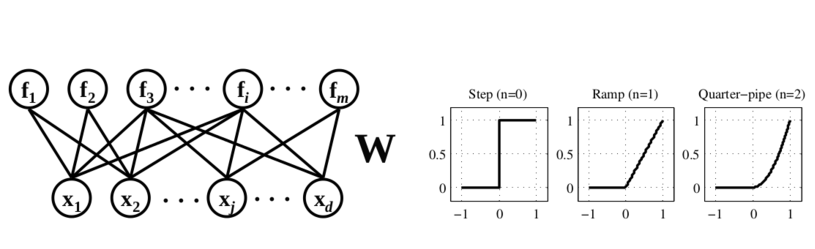
\includegraphics[width=1.0\linewidth, height=7cm]{figures/singnet}
  \caption{Single layer network and thresholded activation functions(\cite{saul} et al.)}
  \label{fig_singnet}
\end{figure}

Let $f(x)$ and $f(y)$ be the outputs corresponding to inputs $x$ and $y$. Then the inner product of $f(x)$ and $f(y)$ is
\[ f(x)\cdot f(y) = \sum_{i=1}^m \Theta(w_i\cdot x) \Theta(w_i\cdot y)(w_i\cdot x)^n (w_i\cdot y)^n\]
Here $w_i$ is the $i^{th}$ row of weight matrix $W$ and $m$ is the no of output units. Assume $W_{ij}$ are Gaussian distributed with zero mean and unit variance and the network has an infinite number of output units. Then
\[ lim_{m\rightarrow \infty} \frac{2}{m}f(x)\cdot f(y) = k_n(x,y) \]
where
\begin{equation}
k_n(x,y) = 2\int dw \frac{e^{-\frac{\norm{w}^2}{2}}}{(2\pi )^{d/2}} \Theta (w\cdot x) \Theta (w\cdot y) (w\cdot x)^n (w\cdot y)^n 
\label{arc_cosine_integral}
\end{equation}
The kernel function obtained in equation \ref{arc_cosine_integral} can be converted into an alternate form as in equation \ref{arc_cosine_kernel} with the derivation shown in \cite{saul} et al.

The multi-layer composition of arc-cosine kernel can be recursively computed as
\[ k^{(L+1)}_n(x,y) = \frac{1}{\Pi} \Bigg[ k^{(L)}(x,x) \textrm{ } k^{(L)}(y,y)\Bigg]^{\frac{n}{2}} J_n(\theta_n^{(L)}) \]
where $\theta_n^{(L)}$ is the angle between images of $x \textrm{ and } y$ in the feature space after L layer composition
\[ \theta_n^{(L)} = \textrm{cos}^{-1}\Bigg( k^{(L)}(x,y) \Bigg[ k^{(L)}(x,x) \textrm{ } k^{(L)}(y,y)\Bigg]^{\frac{-1}{2}} \Bigg) \]
In the above formulation, we have assumed that the arc-cosine kernels have the same degree $n$ at every layers of recursion. We can also use kernels of different degree at different layers. The intuition behind the multi-layer composition in case of arc-cosine kernels is, if the base kernel $k(x,y) = \phi(x) \cdot \phi(y)$ can mimic the computation of a single-layer network, then the iterated mapping in $k^{(L)}(x,y)$ can mimic the computation of multi-layer network(\cite{saul} et al.).

\subsection{MKM Architecture}
 The architecture of MKMs for solving classification tasks  is similar to that of neural network based deep learning machines, with unsupervised feature extraction(using Kernel PCA, \cite{kpca} et al.) followed by supervised feature selection in each layer. Figure \ref{fig_mkm} shows the architecture of an MKM consisting of $L$ layers of non-linear transformations.

\begin{figure}[h]
  \centering
  \captionsetup{justification=centering,margin=0.1cm}
  \includegraphics[scale=0.5]{figures/mkm}
  \caption{An MKM with L layers of transformations. Each layer consists of unsupervised feature extraction(using kernel PCA) followed by supervised feature selection.}
  \label{fig_mkm}
\end{figure}

The supervised feature selection allows us to retain only those set of features that are most informative for the pattern recognition task. The number of features to be passed to the next layer determines the width of that layer. The optimal layer width is computed by ranking the features based on their importance and selecting the required set of feature with the help of a lightweight classifier (detailed procedure is given in the experiments section). This procedure determines the architecture of the network in a greedy, layer-by-layer fashion. In their implementation \cite{saul} et al. used exhaustive search in the range 10 to 300 to determine the optimal set of features. The output from the final layer can be passed to any classifier. Though any kernel can be used for the kernel PCA based feature extraction, \cite{saul} et al. emphasized on using arc-cosine kernels due to their similarity with deep learning architecture of neural networks and the inclusion of multiple layers is significant  only in case of arc-cosine kernels.

\section{Experiments on Arc-cosine Kernel MKMs}
\label{chap2_exp}
Empirical study was conducted on four datasets, in which three were created from \cite{mnist} dataset of handwritten digits by adding noise in the background and one was a binary classification problem on shape images. The detailed experimental set up and a short description about datasets used is given below. 
\subsection{Experimental Set-Up}
In the training phase, for each layer we set apart 10000 datapoints for training the model and 2000 datapoints for cross validating kernel parameters. For the kernel PCA we chose 3000 datapoints  from the training set of 10000 images randomly. In each layer after extracting features with KPCA, we train a lightweight classifier like kNN and test the performance on the held out 2000 images. The best kernel parameter was chosen based on this performance values. With that parameter value, we did feature extraction on the entire dataset and then passed it to feature selection module. The feature selection was done by using univariate feature selection method available in \cite{scikit} library. This method produces a ranking of features with a univariate statistical test. Based on this rank we can choose the required number of important features. We chose top 5 percent features based on this rank, since empirically it was giving a consistant performance.

In the final classification stage SVMs with arc-cosine kernels are used. The metric used for comparing the performance is, percentage loss in test dataset. Percentage loss is estimated as
\[ \textrm{loss in percentage} = \Bigg(1 - \frac{\# \textrm{correct classifications}}{\# \textrm{datapoints}} \Bigg) \times 100 \]

\subsection{Mnist-back-rand Dataset}
The \textit{mnist-back-rand} dataset was created by filling the image background with random pixel values. Each pixel value of the background was generated uniformly between 0 and 255. Image size is 28$\times$28 and the dataset contains 12000 training and 50000 testing images.
\subsection{Mnist-back-image Dataset}
The \textit{mnist-back-image} dataset was generated by filling the image background with random image patches. The patches were extracted randomly from a set of 20 images downloaded from the internet. The dataset contains contains 12000 training and 50000 testing images, each of size 28$\times$28.
\subsection{Mnist-rot-back-image Dataset}
The \textit{mnist-rot-back-image} is a rotated variant of \textit{mnist-back-image} where the rotation angle is generated uniformly between $0$ and $2\pi$. Image size and number of samples are also the same as \textit{mnist-back-image} dataset.
\subsection{Rectangles-image Dataset}
For \textit{rectangles-image} dataset, the classification task is to identify whether a rectangle contained in an image has larger width or length. The dataset is constructed by uniformly sampling the height and width of the rectangles. Then random image patches are added in the background, where image patches are extracted from one of the 20 images used by \textit{mnist-back-image}. Each image is of size 28$\times$28 and each dataset contains 12000 training images and 50000 testing images.

Figure \ref{samples} contains some sample images from first three dataset and Figure \ref{chap2_rect} contains the samples from \textit{rectangles-image} dataset.
\begin{figure}[h]
  \centering
  \captionsetup{justification=centering,margin=0.1cm}
  \includegraphics[scale=0.55]{figures/data_sample1}
  \caption{sample images from \textit{mnist-back-rand}(first row), \textit{mnist-back-image}(second row) and \textit{mnist-rot-back-image}(third row) datasets.}
  \label{samples}
\end{figure}

\begin{figure}[h]
  \centering
  \captionsetup{justification=centering,margin=0.1cm}
  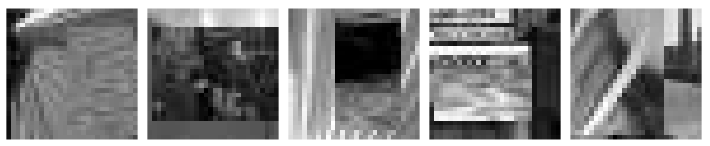
\includegraphics[scale=0.55]{figures/rect_image}
  \caption{sample images from \textit{rectangles-image} dataset.}
  \label{chap2_rect}
\end{figure}

\subsection{Results and Analysis}
\renewcommand{\arraystretch}{2.1}
\begin{table*}
\centering
\begin{tabular}{|c|c|c|c|c|c|c|c|}
  \hline
  \multirow{2}{*}{\textbf{Dataset}} & \multicolumn{7}{ |c| }{\textbf{Loss in Percentage}} \\
  \cline{2-8}
  & $\textrm{SVM}_{\textrm{RBF}}$ & $\textrm{SVM}_{\textrm{Poly}}$ & NNet & DBN-3 & SAA-3 & DBN-1 & MKMs\\
  \hline  
  \textit{back-rand} & 14.58 & 16.62 & 20.04 & \textbf{6.73} & 11.28 & 9.80 & 10.55\\
  \hline
  \textit{back-image} & 22.61 & 24.01 & 27.41 & 16.31 & 23.00 & \textbf{16.15} & 21.39\\
  \hline
  \textit{rot-back-image} & 55.18 & 56.41 & 62.16 & \textbf{47.39} & 51.93 & 52.21 & 51.61\\
  \hline
  \textit{rect-image} & 24.04 & 24.05 & 33.20 & 23.69 & 24.05 & \textbf{22.50} & 23.01\\
  \hline
\end{tabular}
\caption{Experimental Results of MKMs with Arc-cosine Kernels}
\label{tab_results_mkm}
\end{table*}
\renewcommand{\arraystretch}{1}

Table \ref{tab_results_mkm} also contains best results obtained from other models(\cite{dbn} et al.) like SVM with RBF kernel($\textrm{SVM}_{\textrm{RBF}}$), SVM with polynomial kenel($\textrm{SVM}_{\textrm{Poly}}$), single hidden layer feed-forward neural network(NNet\nomenclature{NNet}{Neural Network with one hidden layer}), Deep Belif Networks(DBN)\nomenclature{DBN}{Deep Belif Networks} with 1 hidden layer(DBN-1), DBN with 3 hidden layer(DBN-3) and 3 hidden layer Stacked Autoassociator Network(SAA-3). The first three models comes under shallow architectures and the remaining are deep architectures. From the table, it can be observed that MKMs outperforms all the remaining models except Deep Belif Networks(DBN). Compared to DBN the architecture, parameter tuning and optimization  are fairly simple in MKMs.

The change in the performance of the classifier when each adding layer to the model was also analyzed. Figures \ref{mkm_rand} and \ref{mkm_image} shows the variations in the classifier performance when model complexity was increased by adding more layers(on \textit{mnist-back-rand} and \textit{mnist-back-image} datasets respectively). The results indicates that in some cases better representation can be obtained even with a less complex model (eg: in case of \textit{mnist-back-image} dataset, where the performance degrades when model complexity increases).


\begin{figure}
  \centering
  \captionsetup{justification=centering,margin=0.1cm}
  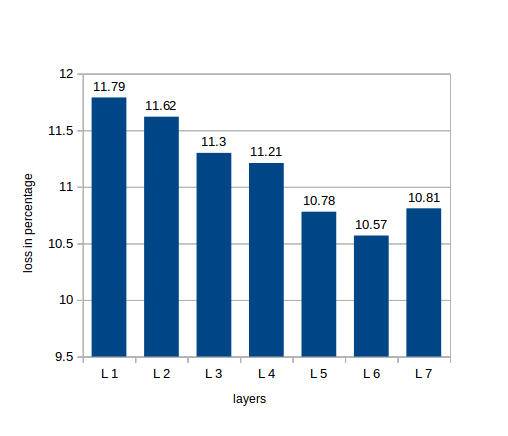
\includegraphics[scale=0.65]{figures/mkm_rand}
  \caption{Change in classifier performance on \textit{mnist-back-rand} dataset when increasing the number of layers.}
  \label{mkm_rand}
\end{figure}

\begin{figure}
  \centering
  \captionsetup{justification=centering,margin=0.1cm}
  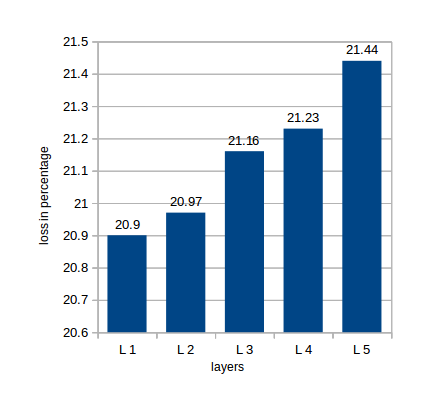
\includegraphics[scale=0.65]{figures/mkm_image}
  \caption{Change in classifier performance on \textit{mnist-back-image} dataset when increasing the number of layers.}
  \label{mkm_image}
\end{figure}

\section{Visualizing Features using tSNE}
\label{chap2_tsne}
In order to visualize the features learned by the MKM, t-distributed Stochastic Neighbor Embedding(tSNE, proposed by \cite{tsne} et al.) was used. tSNE\nomenclature{tSNE}{t-distributed Stochastic Neighbur Embedding} is a tool for visualizing high-dimensional data. It converts the similarities between datapoints to joint probabilities and tries to minimize the Kullback-Leibler divergence(KL divergence) between the joint probabilities of the low-dimensional embedding and the high dimensional data(\cite{tsne} et al.). tSNE is a variant of stochastic neighbor embedding \nomenclature{SNE}, that is much easier to optimize and produce significantly better visualizations by reducing the tendency of the  points to get accumulated  at the center of the map.

Suppose $X = \{x_1, x_2, \ldots, x_n\}$ are the high-dimensional datapoints, and $Y = \{y_1, y_2, \ldots, y_n\}$ the corresponding low-dimensional map points. In SNE, we first convert high-dimensional representation of datapoints into pairwise similarities that can be interpreted as conditional probabilities. Intuitively, the similarity of a datapoint $x_i$ to $x_j$ is interpreted as the probability of $x_i$ picking up $x_j$ as its neighbor with a Gaussian centered at $x_i$(denoted as $p_{j/i}$). Mathematically this is formulated as
\[ p_{j/i} = \frac{exp(-\norm{x_i-x_j}^2/2 \sigma_i^2}{\sum_{k\neq i} exp(-\norm{x_i - x_k}^2/2 \sigma_i^2)}  \]

where $\sigma_i$ is the variance of the Gaussian centered at $x_i$. For every $x_i$ we calculate corresponding $\sigma_i$ which will vary according to the density of datapoints around $x_i$(if the region around $x_i$ is dense $\sigma_i$ will be low and vice versa).

Similarly for the low-dimensional representations $y_i$ and $y_j$ corresponding to $x_i$ and $x_j$ respectively, we compute the conditional probability(denoted as $q_{j/i}$) by setting the variance of the Gaussian to $\frac{1}{\sqrt{2}}$. Thus
\[ q_{j/i} = \frac{exp(-\norm{y_i-y_j}^2}{\sum_{k\neq i} exp(-\norm{y_i - y_k}^2)}  \]

Since we are only interested in modelling pairwise similarity, we set $p_{i/i} = q_{i/i} = 0$. The crux of SNE as stated by \cite{tsne} et al. is ``if the map points $y_i$ and $y_j$ correctly model the similarity between high-dimensional datapoints $x_i$ and $x_j$ then the conditional probabilities $p_{j/i}$ and $q_{j/i}$ will be equal''. In this case, the cost function can be formulated to minimize the difference between conditional probabilities $p_{j/i}$ and $q_{j/i}$ using KL divergence. The cost function $C$ is defined as
\begin{equation}
C = \sum_{i}\textrm{KL}(\textrm{P}_i \big|\big| \textrm{Q}_i) = \sum_{i}\sum_{j} p_{j/i} log \frac{p_{j/i}}{q_{j/i}}
\label{cost_tsne}
\end{equation}
where $\textrm{P}_i$ is the conditional probability distribution over all other datapoints given datapoint $x_i$ and $\textrm{Q}_i$ is the conditional probability distribution over all other map points given the map point $y_i$.

The minimization of the cost function in \ref{cost_tsne} is performed by using gradient descent method. The gradient is computed as
\[ \frac{\partial C}{\partial y_i} = 2\sum_j(p_{j/i}-q_{j/i} + p_{i/j}-q_{i/j})(y_i - y_j) \]
Though SNE can produce good quality visualizations, it has the following limitations.
\begin{itemize}
\item Since the KL divergence is not symmetric, different types of error in the pairwise distances in low-dimensional map are not weighted equally(there is a large cost for using widely separated map points to represent nearby datapoints, but the cost is small for using nearby map points to represent widely separated datapoints).
\item crowding of map points in the center of the map.
\end{itemize}

tSNE is a variant of SNE which improves the visualization quality by alleviating the above mentioned problems.
\begin{itemize}
\item It uses a symmetric version of the SNE cost function by employing a joint probability distribution instead of the conditional probability distribution used by SNE. This also results in simpler gradients.
\item It uses student-t distribution to compute the similarity between map points. tSNE employs a heavy-tailed distribution for the map points to alleviate both the crowding problem and optimization problems of SNE.
\end{itemize}

In the symmetric version of the  tSNE the cost function is computed as shown below.
\begin{equation*}
C = \textrm{KL}(\textrm{P} \big|\big| \textrm{Q}) = \sum_{i}\sum_{j} p_{ij} log \frac{p_{ij}}{q_{ij}}
\end{equation*}
where $P$ and $Q$ are the joint probability distribution functions in the high-dimensional and low-dimensional space respectively. Here also we set $p_{ii}$ and $q_{ii}$ to zero. The symmetry in the cost function is achieved due to the fact that $p_{ij} = p_{ji}$ and $q_{ij} = q_{ji}$ $\forall i,j$. The joint probability in high-dimensional space($p_{ij}$) and low-dimensional space($q_{ij}$) are computed as
\[ p_{ij} = \frac{exp(-\norm{x_i-x_j}^2/2 \sigma^2}{\sum_{k\neq l} exp(-\norm{x_k - x_l}^2/2 \sigma^2)}  \]
\[ q_{ij} = \frac{exp(-\norm{y_i-y_j}^2}{\sum_{k\neq l} exp(-\norm{y_k - y_l}^2)}  \]
The gradient of the symmetric SNE has a fairly simple form
\[ \frac{\partial C}{\partial y_i} = 4\sum_j(p_{ij}-q_{ij})(y_i - y_j) \]
Symmetric SNE still faces problems when a datapoint $x_i$ is an outlier; when $x_i$ is an outlier $\norm{x_i-x_j}^2$ is large for all $x_j$ with $x_i$, hence $p_{ij}$ are extremely low, so the location of its low-dimensional map point $y_i$ has very little effect on the cost function. This problem is addressed in tSNE by defining $p_{ij} = \frac{p_{j/i} + p_{i/j}}{2n}$, which ensures that $\sum_j p_{ij} \ge \frac{1}{2n}$ $\forall \textrm{ } x_i$, hence each datapoint $x_i$ makes a significant contribution to the cost function. The crowding problem is addressed in tSNE by using a student t-distribution with one degree of freedom as the heavy-tailed distribution in the low-dimensional map. Thus the joint probability $q_{ij}$ is computed as
\[ q_{ij} = \frac{(1+\norm{y_i-y_j}^2)^-1}{\sum_{k \neq l} (1+\norm{y_k-y_l}^2)^-1} \] 
Then, finally the gradient of the cost function is obtained as
\[ \frac{\partial C}{\partial y_i} = 4\sum_j(p_{ij}-q_{ij})(y_i - y_j)(1+\norm{y_i-y_j}^2)^-1) \]

tSNE was employed in our experiments to understand the changes in the data distribution before and after the feature learning process. Figure \ref{tsne_rand_raw} shows the tSNE embedding of the raw data from \textit{mnist-back-rand} dataset and figure \ref{tsne_rand_mkm} shows the same embedding applied on the features produced by MKM with arc-cosine kernels. The tSNE embedding of features learned by MKMs are crowded near the center, hence it was difficult to interpret the separability.

\begin{sidewaysfigure}
  \centering
  \captionsetup{justification=centering,margin=0.1cm}
  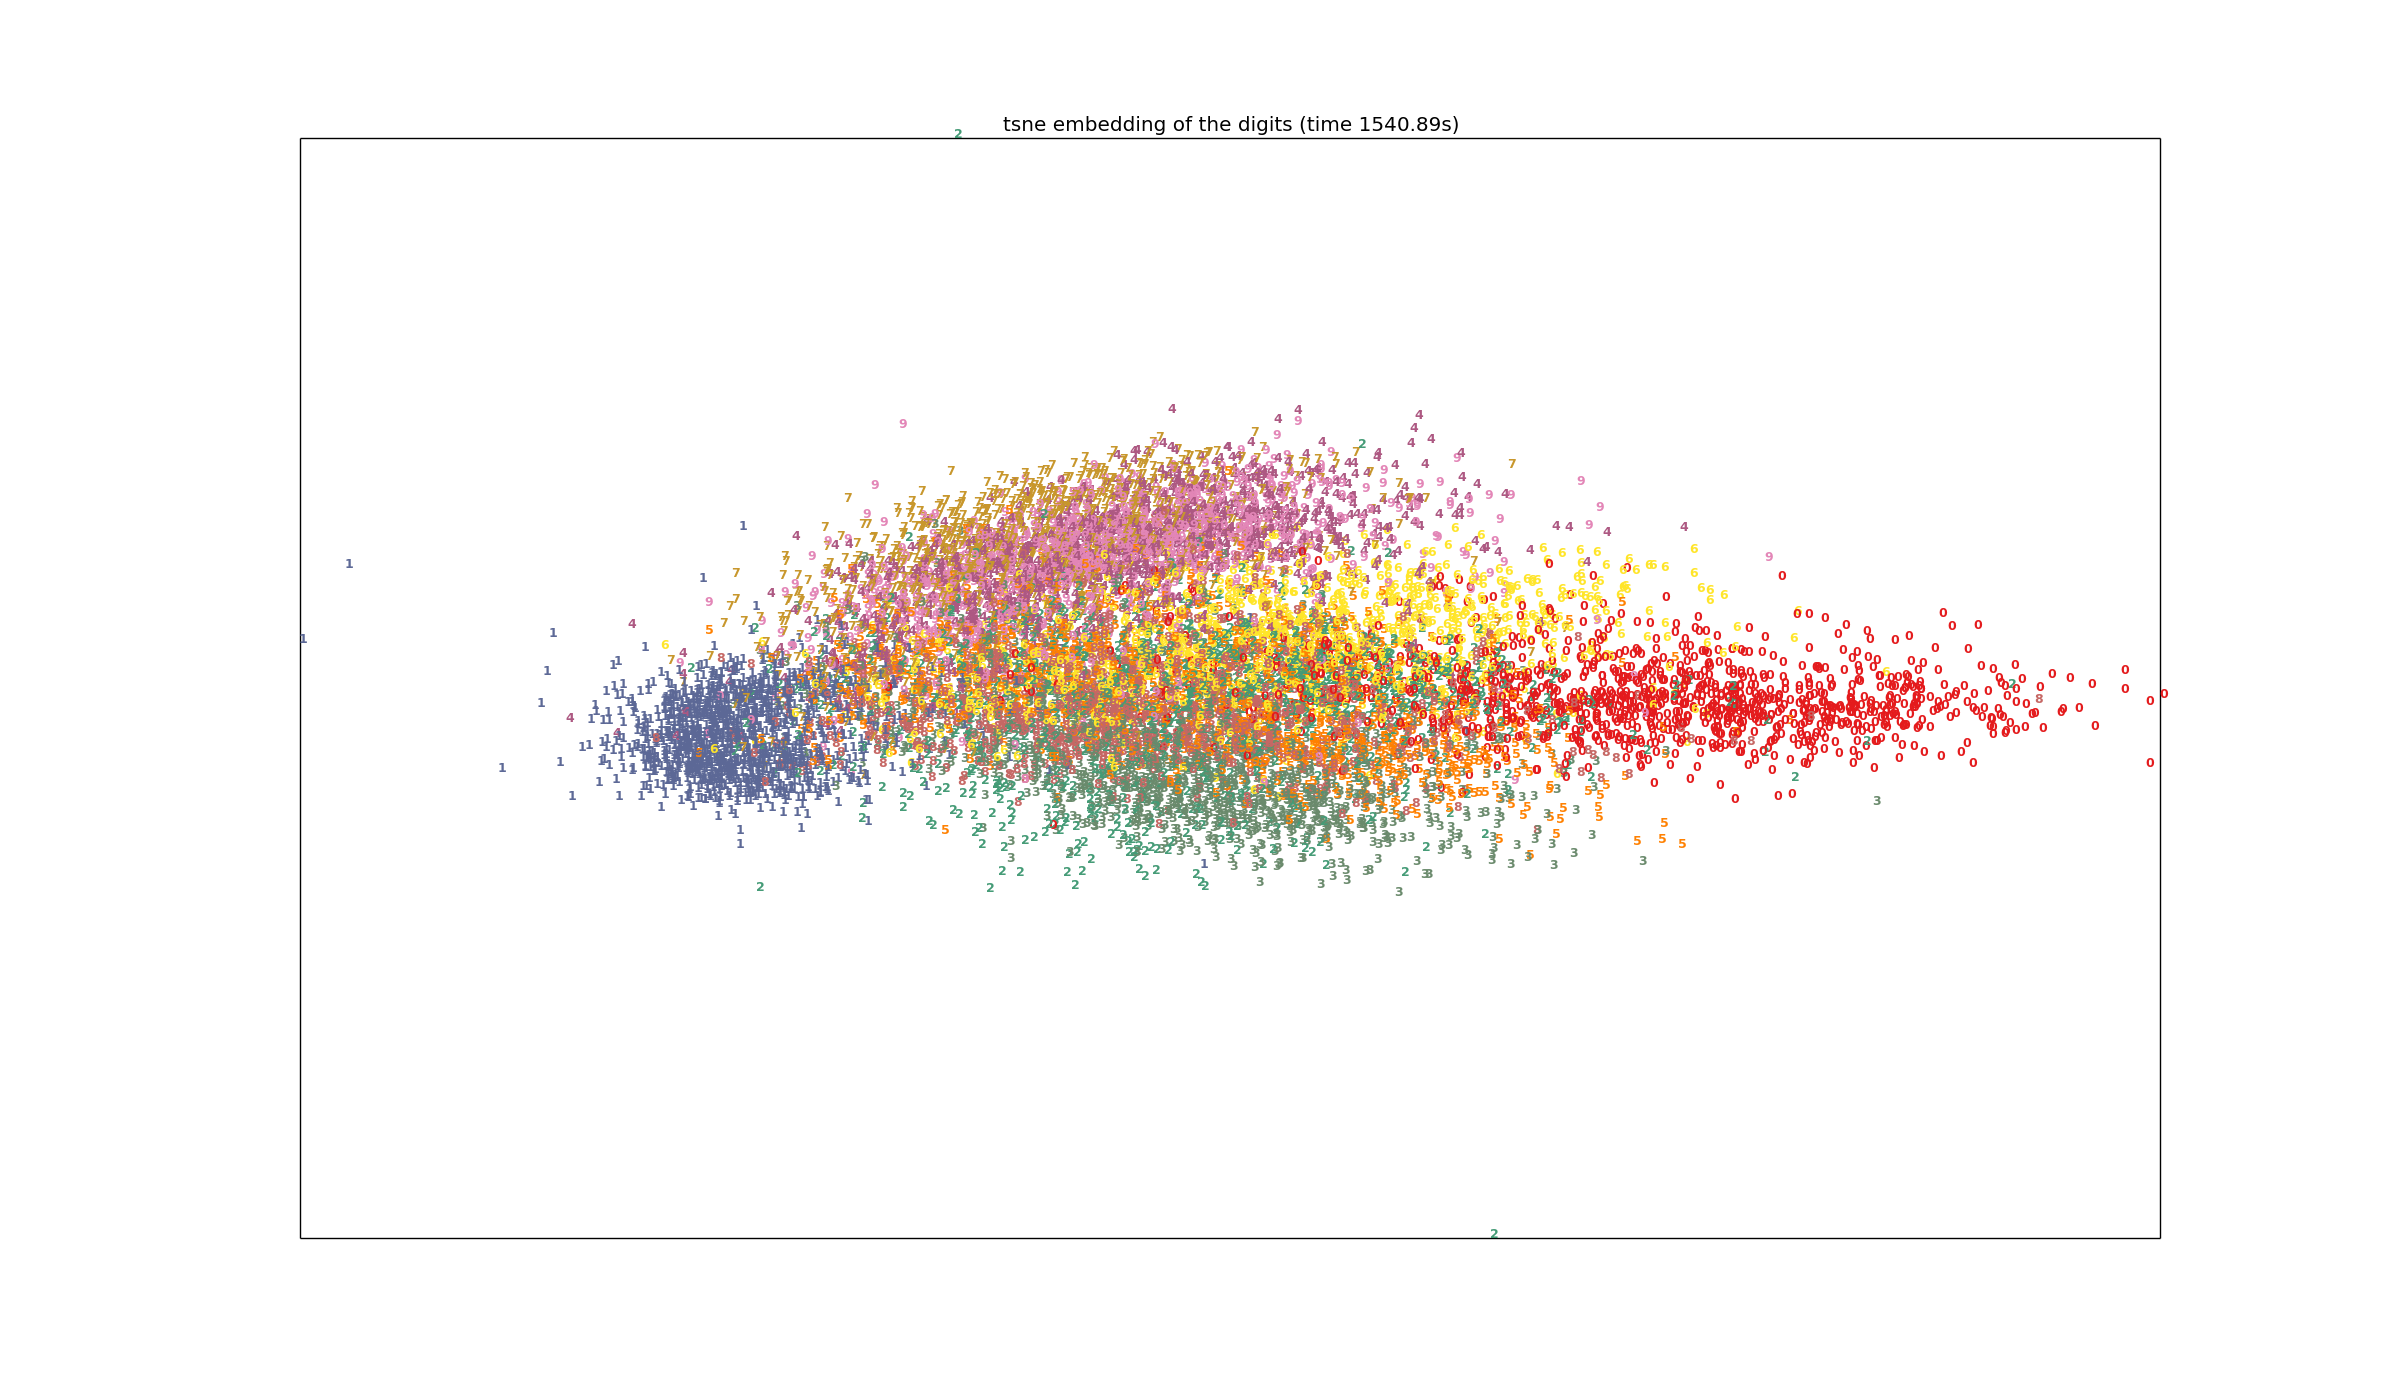
\includegraphics[scale=0.45]{figures/tsne_rand_rawdata}
  \caption{tSNE embedding of raw data from \textit{mnist-back-rand} dataset.}
  \label{tsne_rand_raw}
\end{sidewaysfigure}


\begin{sidewaysfigure}
  \centering
  \captionsetup{justification=centering,margin=0.1cm}
  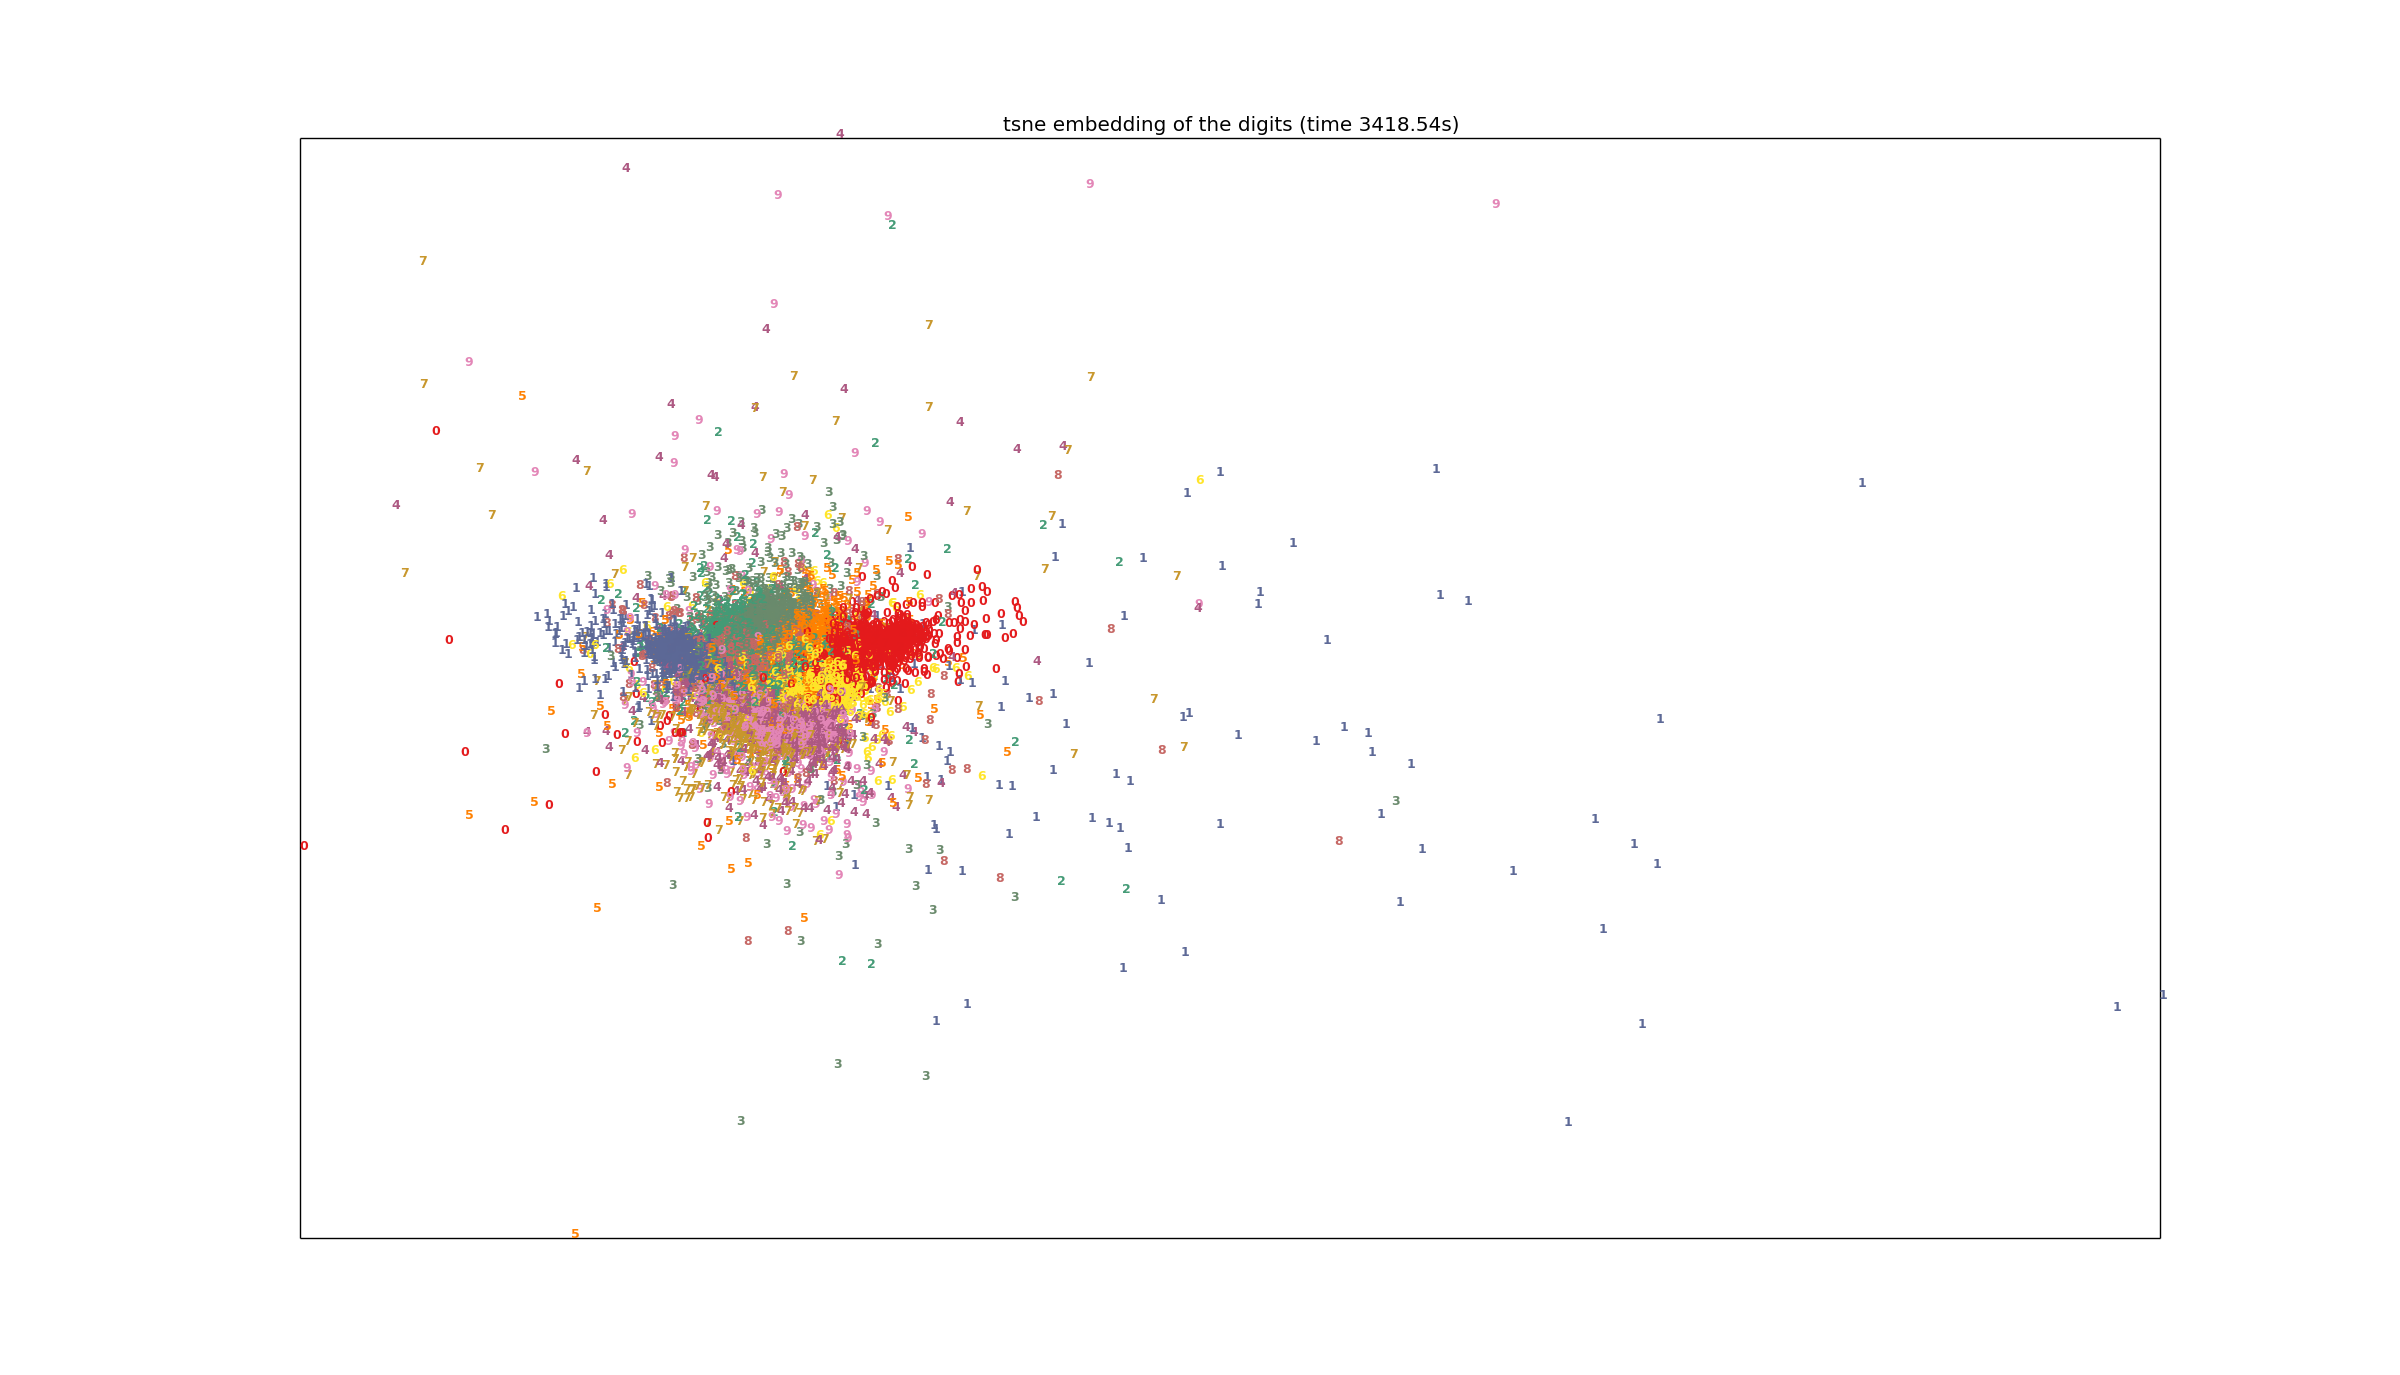
\includegraphics[scale=0.45]{figures/tsne_rand_mkmbest}
  \caption{tSNE embedding of features obtained by MKM from \textit{mnist-back-rand} dataset.}
  \label{tsne_rand_mkm}
\end{sidewaysfigure}



\section{MKMs with Mixed Kernels}
\label{chap2_mkm_mix}
We tried different kernel functions in different layers of MKMs (Gaussian, arc-cosine, polynomial etc.) while performing KPCA. It had been seen that mixing a layer of Gaussian or polynomial kernel in between successive layers of arc-cosine kernel improves the result. This further supported the belief that, with more similarity information (by using more kernels) in hand, we can build better representations. Table \ref{tab_results_mix} shows the result obtained with the mixed kernel models. Because of the improved performance, we used  Multi-layer Multiple Kernel Machines(ML-MKL) model for our analysis, whose  discussion is given in the next chapter.

\renewcommand{\arraystretch}{2.1}
\begin{table}
\centering
\begin{tabular}{|c|c|c|c|c|c|c|c|}
  \hline
  \multirow{2}{*}{\textbf{Dataset}} & \multicolumn{7}{ |c| }{\textbf{Loss in Percentage}} \\
  \cline{2-8}
  & $\textrm{SVM}_{\textrm{RBF}}$ & $\textrm{SVM}_{\textrm{Poly}}$ & NNet & DBN-3 & SAA-3 & DBN-1 & $\textrm{MKMs}_\textrm{(mix)}$\\
  \hline  
  \textit{back-rand} & 14.58 & 16.62 & 20.04 & \textbf{6.73} & 11.28 & 9.80 & 9.54\\
  \hline
  \textit{back-image} & 22.61 & 24.01 & 27.41 & 16.31 & 23.00 & \textbf{16.15} & 20.94\\
  \hline
  \textit{rot-back-image} & 55.18 & 56.41 & 62.16 & \textbf{47.39} & 51.93 & 52.21 & 54.03\\
  \hline
  \textit{rect-image} & 24.04 & 24.05 & 33.20 & 23.69 & 24.05 & \textbf{22.50} & 25.04\\
  \hline
\end{tabular}
\caption{Experimental Results of MKMs with Mixed Kernels}
\label{tab_results_mix}
\end{table}
\renewcommand{\arraystretch}{1}

As in MKMs with arc-cosine kernel, we chose top 5 percent features based on univariate test score for the mixed kernel MKMs. The classifier used in the output layer was an SVM\nomenclature{SVM}{Support Vector Machines} with arc-cosine kernel. The results indicates that MKMs with mixed kernels improved the classifier performance for \textit{mnist-back-rand} and \textit{mnist-back-image} datasets, whereas the classification accuracy declined in the case of \textit{mnist-rot-back-image} and \textit{rectangles-image} dataset. The tSNE embedding of the features produced by MKMs with mixed kernels is shown in figure \ref{tsne_rand_mkmmix} (for \textit{mnist-back-rand} dataset). The best result in this dataset was obtained from a model consisting of three layers with a Gaussian kernel in the middle layer. The visualization indicates that, MKMs with mixed kernels has good separability between different classes.
\begin{sidewaysfigure}
  \centering
  \captionsetup{justification=centering,margin=0.1cm}
  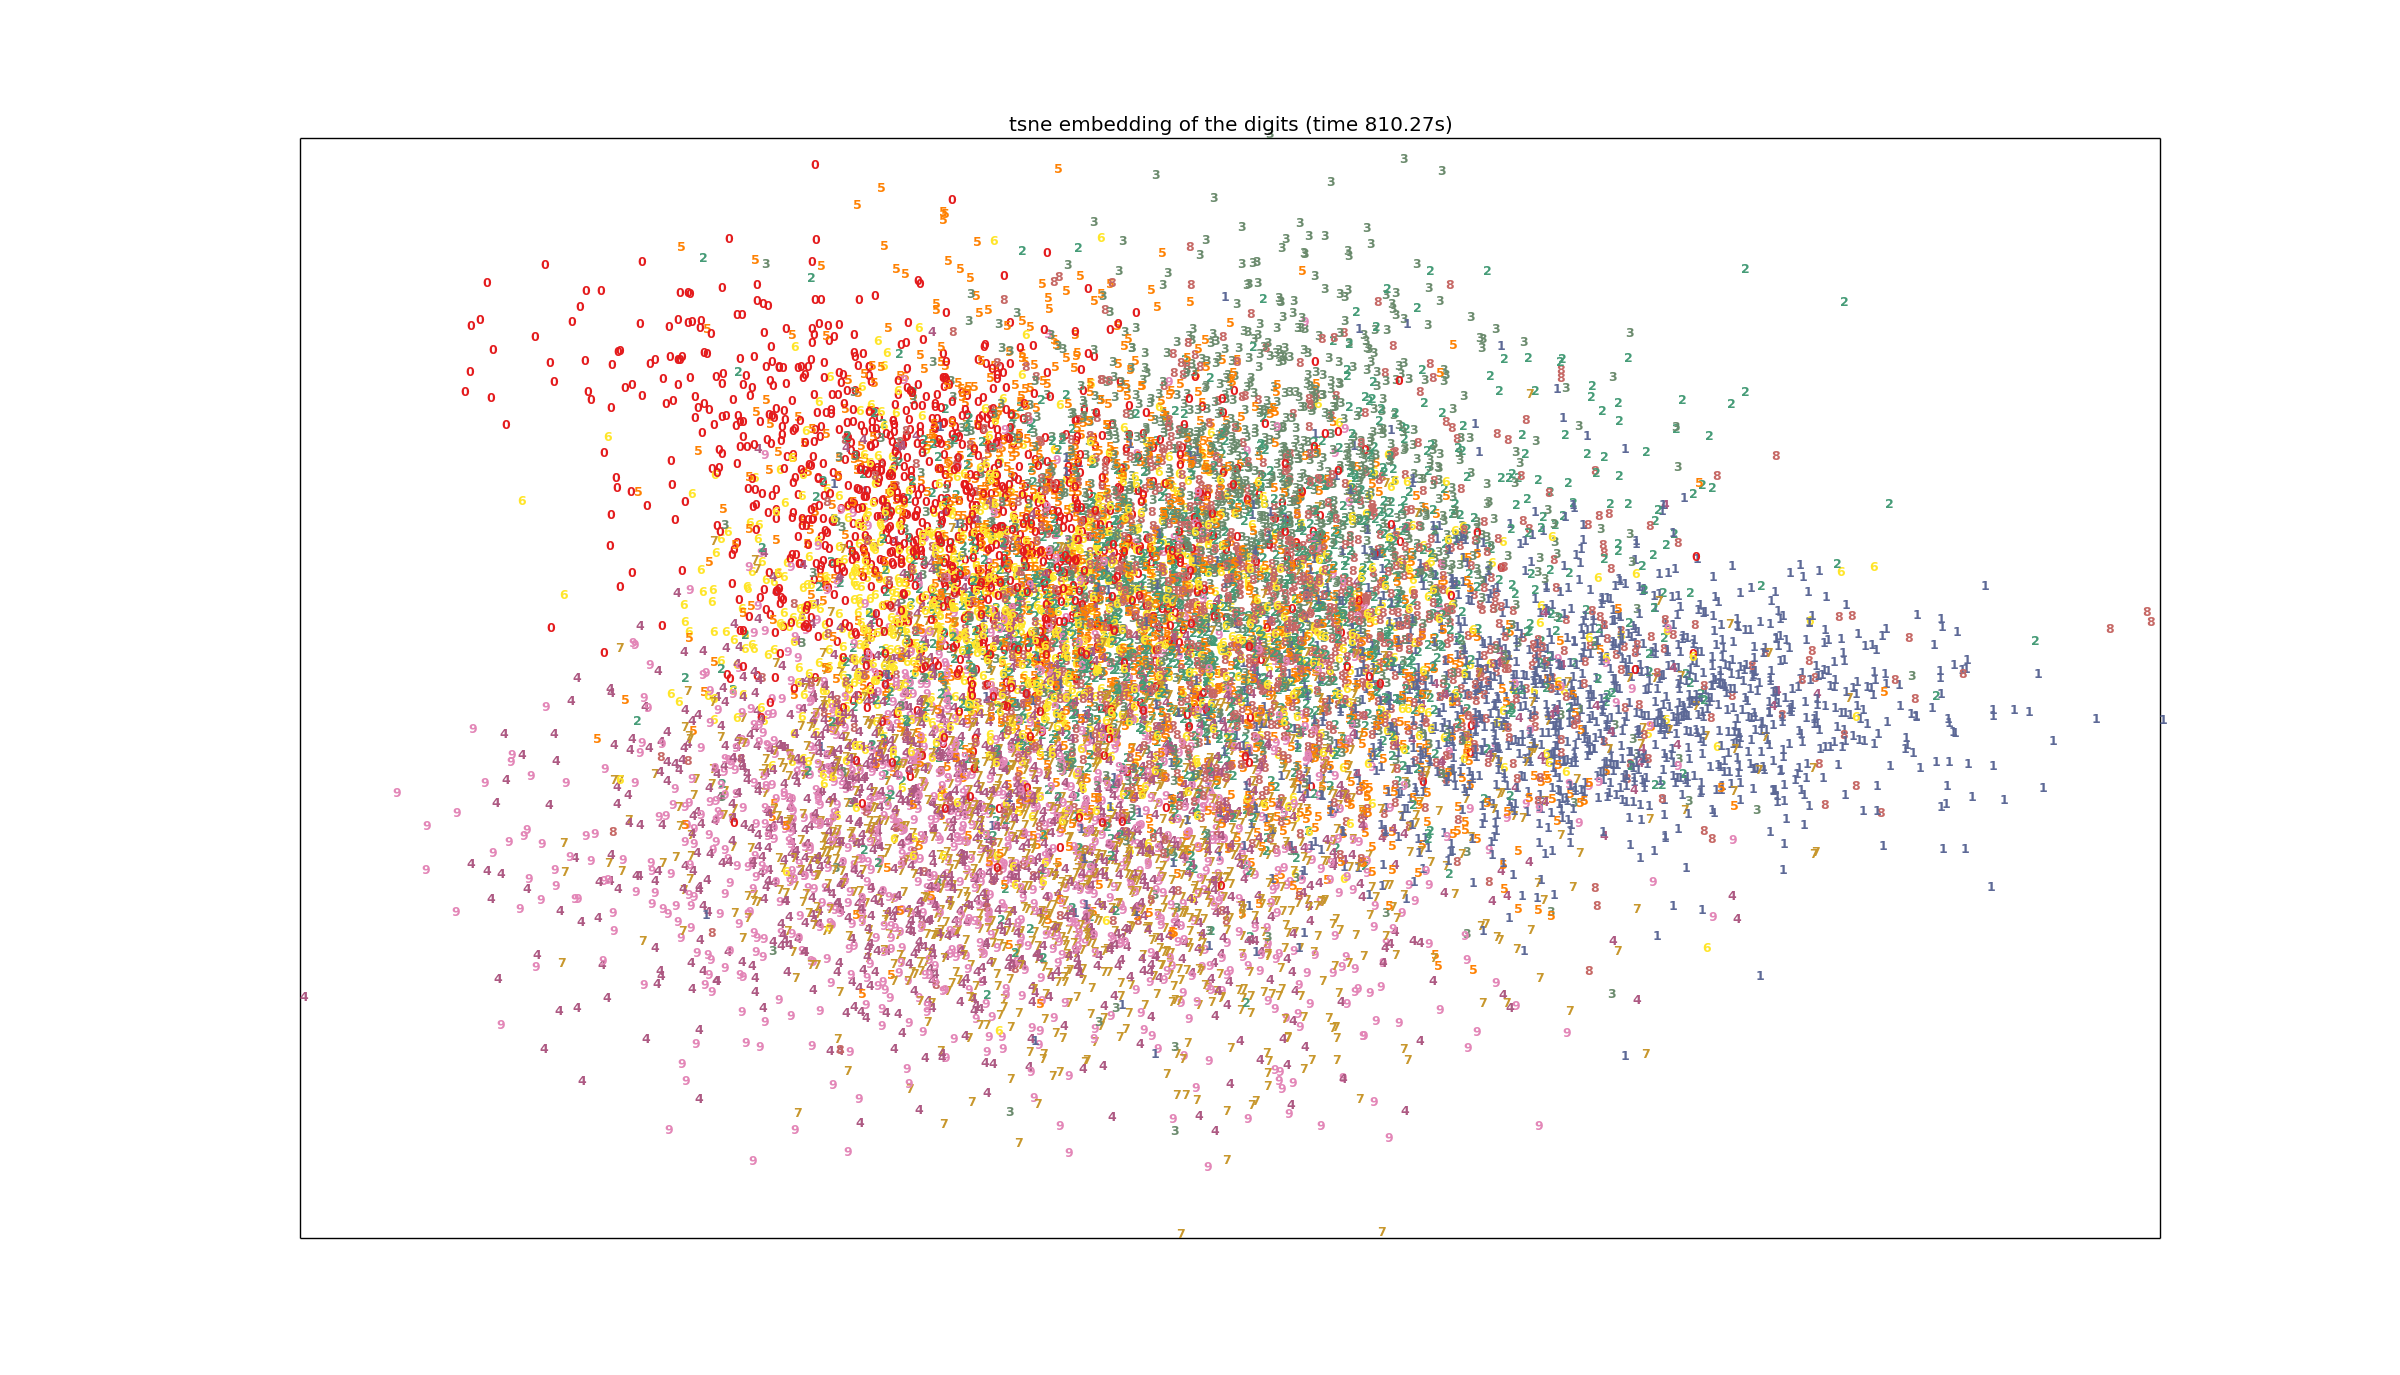
\includegraphics[scale=0.45]{figures/tsne_rand_mkmmix}
  \caption{tSNE embedding of features obtained by MKM with mixed kernels from \textit{mnist-back-rand} dataset.}
  \label{tsne_rand_mkmmix}
\end{sidewaysfigure}


\section{Conclusion}
\label{chap2_conc}
In this chapter we analysed the MKMs framework which has the characteristics of deep learning algorithms by employing  kernel methods. The empirical study indicated that MKMs are performing comparable with that of  popular deep learning algorithms like DBN, SAA etc. We also analysed the performnace of MKMs with mixed kernels. The mixing produces better results when other kernels are sandwiched between two arc-cosine kernels.

The visualization of features learned by MKMs are difficult to interpret due to crowding of datapoints near the center, but for MKMs with mixed kernels the visualization indicates that the separation is good enough between different classes, even though the samples from same class is distributed in different locations.
 % unbounded cylinder

\chapter{Multi-layer Multiple Kernel Learning}
\label{chap_mlmkl}
In this chapter we  discuss the Multi-layer Multiple Kernel Learning (ML-MKL\nomenclature{ML-MKL}{Multi-layer Multiple Kernel Learning}) framework developed using an unsupervised MKL algorithm. The organization of this chapter is as follows;  section \ref{sec_mkl} gives  the discussion of  traditional MKL algorithm  in a supervised learning settings, in section \ref{sec_umkl} the unsupervised MKL formulation is introduced, in section \ref{sec_rw} the related works in ML-MKL domain is discussed, in section \ref{sec_mlmkl} the proposed ML-MKL algorithm is discussed along with the experimental results and section \ref{sec_conc} concludes this chapter.


\section{Multiple Kernel Learning}
\label{sec_mkl}
Multiple Kernel Learning(MKL\nomenclature{MKL}{Multiple Kernel Learning}) aims at learning a convex combination of a set of predefined base kernels for choosing an optimum kernel(\cite{mkl} et al.). The primary aim of MKL algorithm is to automate the process of choosing the optimum kernel  for the learning task.


Typically multiple kernel learning is formulated in a supervised learning settings. Suppose we are given $n$ datapoints $\mathcal{D} = \{(x_1, y_1), (x_2, y_2), \ldots, (x_n, y_n)\}$, where $x_i \in \mathbb{R}^d$ is the $i^{th}$ input data vector and $y_i$ is the label of the class to which $x_i$ belongs to. Then the MKL learning task is formulated as the following optimization problem.
\begin{equation}
\min_{k \in \mathcal{K}} \min_{f \in \mathcal{H}_k} \lambda \norm{f}^2_{\mathcal{H}_k} + \sum_{i=1}^n l(y_i, f(x_i))
\end{equation}
where $l(\cdot)$ denotes the loss function(commonly used loss function is the hinge loss, defined as $l(t) = \max(0, 1-t)$), $\mathcal{H}_k$ is the RKHS corresponding to the kernel $k$, $\mathcal{K}$ denotes the optimization domain of the candidate kernels, and $\lambda > 0$ is the regularization parameter.

The optimizaion domain $\mathcal{K}$ is the convex combination of a set of predefined base kernels, defined as follows
\[ \mathcal{K} = \Bigg\{ k( \cdot \textrm{ , } \cdot ) = \sum_{t=1}^m \mu_t k_t(\cdot \textrm{ , } \cdot) \textrm{ : } \sum_{t=1}^m \mu_t = 1, \mu_t \geq 0 \Bigg\} \]
where $k_t$ is the $t^{th}$ base kernel and $\mu_t$ is the weight associated to the $t^{th}$ base kernel. The decision function $f(x)$ can be computed as a linear combination of kernel evaluations on all training samples;
\[ f(x) = \sum_{i=1}^n \alpha_i k(x_i, x) \]
where $\alpha_i$'s are the coefficients. As per the definition of kernel $k$ in MKL, the decision function of the conventional MKL is expressed as
\begin{equation*}
\begin{aligned}
f(x) &= \sum_{i=1}^n \alpha_i \sum_{t=1}^m \mu_t k_t(x_i, x) \\
&= \sum_{i=1}^n \sum_{t=1}^m \alpha_i \mu_t k_t(x_i, x)
\end{aligned}
\end{equation*}
In this basic formulation, the optimization task has to identify both the optimal kernel $k$ from the domain $\mathcal{K}$ and the optimal decision function $f$ from the RKHS $\mathcal{H}_k$ simultaneously. In order to eliminate this problem \cite{corinna} et al. proposed a two stage kernel learning algorithm which separates the kernel learning task from the decision function learning.


\section{Unsupervised MKL}
\label{sec_umkl}
In the KPCA based feature extraction stages, we were using only one kernel for the task. With the intuition that by using multiple kernels at each layer we would get more similarity information, we computed a convex combination of multiple kernels following the work in \cite{zhuang} et al. Since we are using kernels for unsupervised feature extraction, traditional MKLs following supervised paradigm cannot be used here.

The goal of an unsupervised multiple kernel learning task is to find an optimal linear combination of the $m$ kernel functions as, i.e, $k^*(\cdot \textrm{ , } \cdot) \in \mathcal{K}$. %where $K$ is defined as follows:
%\[ K = \Bigg\{ k( \cdot \textrm{ , } \cdot ) = \sum_{t=1}^m \mu_t k_t(\cdot \textrm{ , } \cdot) \textrm{ : } \sum_{t=1}^m \mu_t = 1, \mu_t \geq 0 \Bigg\} \]  
%here $k_t$'s are the base kernels. 
In order to determine the optimality of a linear combination of kernels, we used the following quality criteria\cite{zhuang} et al.:

\begin{itemize}
\item A  good kernel should enable each training instances to be well reconstructed from the localized bases weighted by the kernel values. Formulating this requirment mathematically, for each $x_i$ we expect the optimal kernel should minimize the approximation error $\norm{x_i-\sum_j k_{ij}x_j}^2$, where $k_{ij} = k(x_i, x_j)$.
\item A good kernel should induce kernel values that are coincided with the local geometry of the training data. This is equivalent to finding the optimal kernel that minimizes the distortion over all trainig data, computed as $\sum_{i,j}k_{ij} \norm{x_i-x_j}^2 $.
\end{itemize}

In addition to this, the locality preserving principle can be exploited  by using a set of local bases for each $x_i \in X$ denoted as $B_i$. By fixing the size of the local bases to some constant $N_B$,  the optimization problem of unsupervised MKL can be formulated as follows.
\[ \min_{k \in \mathcal{K}} \frac{1}{2}\sum_{i=1}^n \norm{x_i - \sum_{x_j \in B_i} k_{ij}x_j}^2 + \gamma* \sum_{i=1}^n \sum_{x_j \in B_i} k_{ij} \norm{x_i-x_j}^2 \]

where $\gamma$ is a tuning parameter, which controls the tradeoff between the coding error and the locality distortion. Converting to matrix notations the above problem becomes
\begin{equation}
  \min_{\mu \in \Delta,D} \frac{1}{2} \norm{X(I-K \circ D)}_F^2 + \gamma* \textrm{ tr }K\circ D\circ M(11^T)
  \label{obj_mat} 
\end{equation}
%\begin{equation*}
 % \begin{aligned}
\[ \textrm{subject to } D \in \{0,1\}^{n \times n} \]
\[  \norm{d_i}_1 = N_B, i=1,2,\ldots,n \]
\[ \Delta = \Big\{\mu : \mu^T\textbf{1} = 1, \mu \geq 0 \Big\} \textrm{ and } \]
\[ [K]_{i,j} = \sum_{t=1}^m \mu_t k^t(x_i, x_j), 1\leq i,j \leq n \]
  %\end{aligned}
%\end{equation*}

The matrix $D \in \{0,1\}^{n \times n}$ contains information about local bases of each $x_i$ as a column vector. In particular, each column vector $d_i \in \{0, 1\}^n $ in $D$ has a 1 at those points $j$ where, $x_j \in B_i$ and zero elsewhere(or $B_i = \{ x_j : d_j \neq 0 \} $). The matrix M is defined as
\[ [M]_{ij} = x_i^Tx_i + x_j^Tx_j - 2x_i^Tx_j \]

In equation \ref{obj_mat} the notation `$\circ$' denotes elementwise multiplication of two matrices, $\norm{\cdot}_F^2$ denotes the Frobenius norm of a matrix and `tr' denotes the trace of a matrix.

In their implementation(\cite{zhuang}) Zhuang et.al solved the optimization problem in two stages in an alternating fashion, first by solving for $\mu$ with a fixed $D$ (using convex optimization) and then solving for $D$ by fixing $\mu$ (using a greedy mixed integer programming formulation). Since we are using a many layer architecture, the alternating optimization strategy is too costly; so we chose to do the optimization across $\mu$ only by choosing $D$ beforehand. Specifically, the matrix $D$ is computed beforehand by taking $k$ nearest neighbours of $x_i$ from the training set and putting a one in those positions for $d_i$. Rest of the positions are filled with zeros. The resulting optimization problem will be  
\begin{equation}
  \begin{aligned}
  \min_{\mu \in \Delta} \frac{1}{2} \norm{X(I-K \circ D)}_F^2 + \gamma* \textrm{ tr }K\circ D\circ M(11^T)
  \end{aligned}
\end{equation}
\[ \textrm{subject to } D \in \{0,1\}^{n \times n}, \norm{d_i}_1 = N_B, i=1,2,\ldots,n \]
\[ \Delta = \Big\{\mu : \mu^T\textbf{1} = 1, \mu \geq 0 \Big\} \]

The objective function can be formulated as a convex quadratic programming problem w.r.t to kernel weights $\mu$ as shown below(derivation of the objective function $J(\mu)$ is shown in Appendix \ref{derivation1}).
\begin{equation}
J(\mu) = \mu^T \Bigg( \sum_{t=1}^m \sum_{i=1}^n k_{t,i}k_{t,i}^T \circ d_i d_i^T \circ P \Bigg)^T \mu + z^T \mu 
\end{equation}
where $[z]_t = \sum_{i=1}^n (2 \gamma v_i \circ d_i - 2 p_i \circ d_i)^T \mathit{k}_{t,i} $, $P = X^TX$, and $\mathit{k}_{t,i} = \Big[ k^t(x_i, x_1), \ldots, k^t(x_i, x_n) \Big]^T $ is the $i^{th}$ column of the $t^{th}$ kernel matrix. $p$ and $v$ are columns of $P$ and $M$ corresponding to $x_i$ respectively.

\section{Related Works}
\label{sec_rw}

\cite{2l_mkl} et al. explored the idea of ML-MKL, in which at each layer they took a non-linear combination of kernels in the previous layer, forming a layered structure. They called such a model as deep multiple kernel learning framework. The architecture of their model is shown in figure \ref{fig_2l_mkl}. The kernel function obtained at layer $l$ is having the following domain.
\[ \mathcal{K}^{(l)} = \bigg\{ k^{(l)}(\cdot, \cdot) = g^{(l)}\Big( \big[k_1^{(l-1)},\ldots, k_m^{(l)}(\cdot, \cdot) \big] \Big)  \bigg\} \]

\begin{figure*}
  \centering
  \captionsetup{justification=centering,margin=0.1cm}
  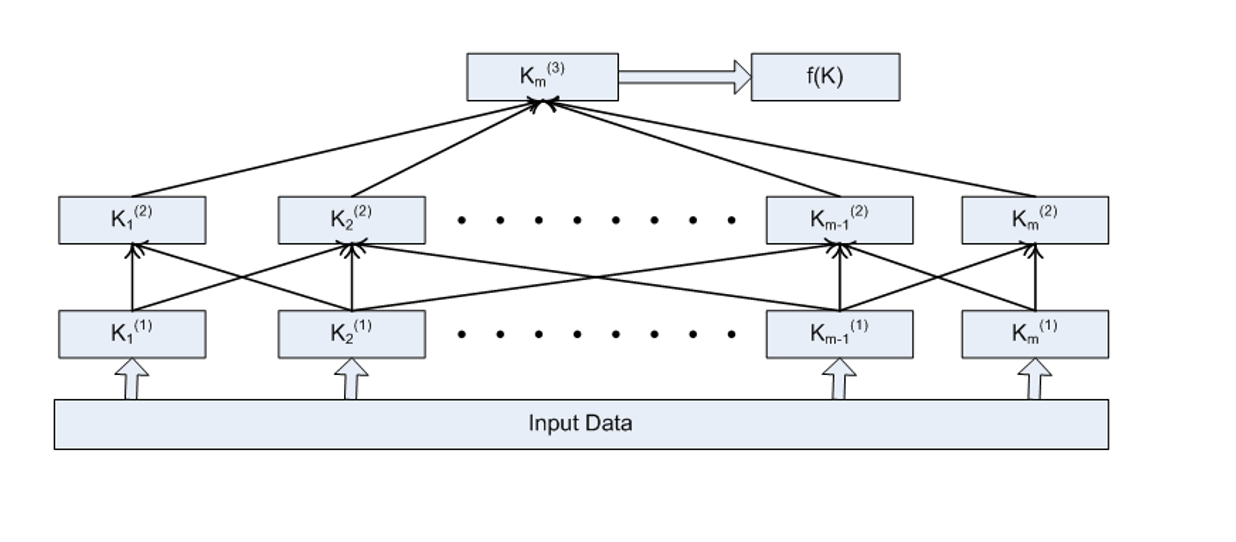
\includegraphics[width=1.1\textwidth,height=8.5cm]{figures/2lmkl}
  \caption{Architecture of ML-MKL model proposed by \cite{2l_mkl} et al.}
  \label{fig_2l_mkl}
\end{figure*}

where $g^{(l)}$ is a function to combine multiple $(l-1)$ level kernels, which must ensure the resulting combination is a valid kernel. Though this combination can be applied for any number of layers, optimization problem is difficult to solve beyond two layers. Hence \cite{2l_mkl} et al. considered only 2-layer MKL in their empirical study. 

In the 2-layer MKL, \cite{2l_mkl} et al. defined the kernel domain by using an RBF kernel for the combination function. 
\[ \mathcal{K}^{(2)} = \bigg\{ k^{(2)}(x_i, x_j;\bm{\mu}) = exp\Big( \sum_{t=1}^m \mu_t k_t^{(1)}(x_i, x_j) \Big)  \bigg\}  \colon \bm{\mu} \in \mathbb{R}_+^m \]
$\mu_t$ is the weight of the $t^{(th)}$ antecedent layer kernel $k_t^{(1)}$(superscript (1) is used here because the antecedent layer is layer 1 in a 2-layer architecture). In order to prevent the kernel weight being too large, the kernel weights are also introduced into the optimization objective as a regularization term. Then the optimization objective becomes
\begin{equation}
\min_{k \in \mathcal{K}} \min_{f \in \mathcal{H}_k} \norm{f}^2_{\mathcal{H}_k} + \mathcal{C} \sum_{i=1}^n l(y_i, f(x_i)) + \sum_{t=1}^m \mu_t
\end{equation}
solving the Lagrangian, we will get the dual objective function as
\[ \min_{\bm{\mu}} \max_{\bm{\alpha}} \sum_{i=1}^n \alpha_i - \frac{1}{2}\sum_{i,j=1}^n \alpha_i \alpha_j y_i y_j k^{(2)}(x_i, x_j;\bm{\mu}) + \sum_{t=1}^m \mu_t \]
\[ \textrm{s.t } 0\leq \alpha_i\leq \mathcal{C}, \sum_{i=1}^n \alpha_i y_i = 0, \mu_t \geq 0, t=1, \ldots, m \]
where $\alpha = [\alpha_1, \alpha_2, \ldots, \alpha_n]^T$ is a vector of dual variables and $\mu = [\mu_1, \mu_2, \ldots, \mu_m]^T$. The final decision function of the 2-layer MKL is given as
\[f(x;\bm{\alpha}, \bm{\mu}) = \sum_{i=1}^n \alpha_i y_i k^{(2)}(x_i, x;\bm{\mu}) + b \]
where $b$ is the bias term. Rewriting the optimization objective in terms of $\alpha$ and $\mu$, we have
\[ \mathcal{J}(\alpha, \mu) = \frac{1}{2} \sum_{i,j=1}^n \alpha_i \alpha_j y_i y_j k^{(2)}(x_i, x_j;\bm{\mu}) - \sum_{i=1}^n \alpha_i - \sum_{t=1}^m \mu_t \]
The optimization problem is solved in two stages
\begin{itemize}
\item by fixing $\mu$ and solve for $\alpha$.
\item by fixing $\alpha$ and solve for $\mu$.
\end{itemize}
Since $k^{(2)}$ is positive definite $\mathcal{J}(\alpha, \mu)$ is convex over $\alpha$, thus an SVM solver can be used to solve the optimization over $\alpha$. The optimization over $\mu$ is solved using gradient ascent. In order to address the challenge of choosing the optimal set of base kernels, they proposed to choose base kernels iteratively inside $k^{(2)}$.

\cite{deep_mkl} et al. used backpropagation algorithm for designing the ML-MKL framework. The architecture of the model studied by them is shown in figure \ref{fig_deep_mkl}. They defined the kernel domain at level $l$ as

\begin{figure*}
  \centering
  \captionsetup{justification=centering,margin=0.1cm}
  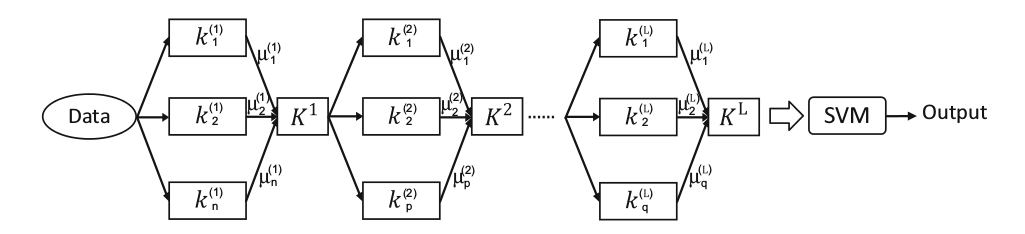
\includegraphics[width=1\textwidth,height=6cm]{figures/back_prop_mlmkl}
  \caption{Architecture of ML-MKL model proposed by \cite{deep_mkl} et al. The kernels in each layer are linearly combined and the resulting Gram matrix is passed to the next layer as input.}
  \label{fig_deep_mkl}
\end{figure*}

\[ \mathcal{K}^{(l)} = \big\{ K^{(l)}(K^{(l-1)}; \mu^{(l)}) = \sum_{t=1}^m \mu_t^{(l)} k_t^{(l)}(K^{(l-1)})  \big\} \]
\[ \textrm{s.t } \mu_t^{(l)} \geq 0, l = 1, \ldots, L \]
where $k_t^{(l)}$ is the $k^{th}$ base kernel at layer $l$ and $\mu_t^{(l)}$ denotes the weight of the $k^{th}$ base kernel at layer $l$. $L$ is the total number of layers. The feature extracted in the antecedent layer are combined linearly and passed to the next layer as input. The kernel weights are obtained by minimizing the mean squre error(denotes as $\mathcal{E}$) of the predicted outputs.
\[ \mathcal{E} = \frac{1}{2n} \sum_{i=1}^n \norm{f(x_i) - y_i}^2 \]
where $f(x_i)$ is the value of the decision function for the input $x_i$, which is computed as
\[ f(x) = \sum_{i=1}^n \alpha_i y_i K^{(l)}(K^{(l-1)}; \mu^{(l)}) + b \]
where $b$ is the bias term. The weights $\mu^{(l)}$ in each layer are obtained using gradient descent algoritm.
\[ \mu^{(l)} := \mu^{(l)} + \eta \nabla \mathcal{E}  \textrm{ } l = 1, \ldots, L \]
\[ \nabla \mathcal{E} = \Bigg\{ \frac{\partial \mathcal{E}}{\partial \mu_1^{(1)}}, \cdots, \frac{\partial \mathcal{E}}{\partial \mu_m^{(1)}}; \cdots; \frac{\partial \mathcal{E}}{\partial \mu_1^{(L)}}, \cdots, \frac{\partial \mathcal{E}}{\partial \mu_m^{(L)}}  \Bigg\}  \]
Here $\eta$ is the learning rate parameter. The error obtained in the final layer are propagated back to all layers using backpropagation algorithm to update the kernel weight parameters $\mu^{(l)}$ in each layer.

\section{Multi-layer Multiple Kernel Learning}
\label{sec_mlmkl}
The architectue of the proposed ML-MKL framework is shown in figure \ref{fig_mlmkl}. It consists of many layers and in each layer the kernel PCA based feature extraction is performed using the combination of a set of predefined kernels. The dimensionality of the features thus obtained are reduced by using supervised feature selection techniques. The final output can be given to any classifier. Algorithm \ref{algo1} summarizes the proposed ML-MKL algorithm.

\begin{algorithm}
\caption{ML-MKL Algorithm}
\textbf{Input}: data X, true labels y, no. of layers L, base kernels for each layer $K_{base}^{(l)} = \{k_1^{(l)}, k_2^{(l)}, k_m^{(l)}\}$, $N_B$, $\gamma$\;
\textbf{Output}: kernel weights $\mu^l$ for each layer, predicted labels\;
1.Initialize $[M]_{ij} = x_i^Tx_i + x_j^Tx_j - 2x_i^Tx_j$, $\bm{D} = d_1, d_2, \ldots, d_n$ as row vectors, where $d_i = \{1 \textrm{ if } x_j \in B_i \textrm{ else } 0 \forall x_j \in X \}$, $\mu = \frac{1}{m}$, $\bm{P} = X^TX$\;
2.\For{each layer l}{
    a. $\bm{W} = \sum_{t=1}^m \sum_{i=1}^n k_{t,i}^{(l)}k_{t,i}^{(l)^{T}} \circ d_i d_i^T \circ P$\\
    b. $\bm{[z]}_t^l = \sum_{i=1}^n (2 \gamma v_i \circ d_i - 2 p_i \circ d_i)^T \mathit{k}_{t,i}^{(l)}$\\
    c. $\bm{\mu}^{*^{l}} = \mu^{l^{T}}W\mu^l + z^{l^{T}}\mu^l$\\
    d. $\bm{K}_{new} = \sum_{t=1}^m \mu_t^l * K_t^{(l)}$\\
    e. extract principal components with $\bm{K}_{new}$\\
    f. select most informative features for layer $l$($X_{new}$)\\
    g. $\bm{P} = X_{new} ^T X_{new}$
}
3.Give the final set of features to any classifier\;
\label{algo1}
\end{algorithm}

\begin{figure*}
  \centering
  \captionsetup{justification=centering,margin=0.1cm}
  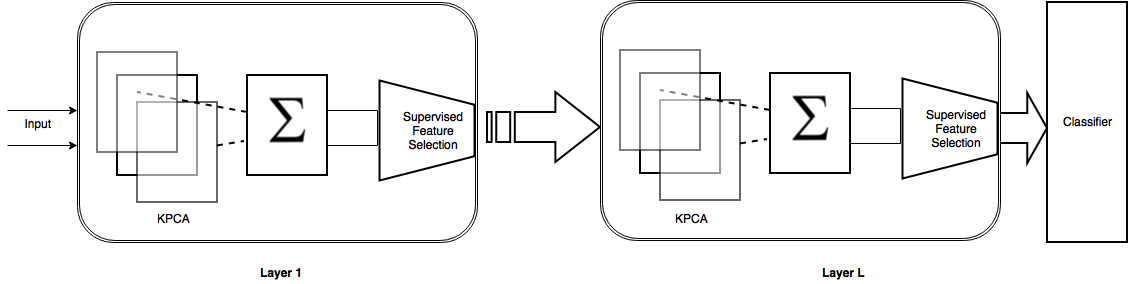
\includegraphics[width=1.0\textwidth,height=5.5cm]{figures/mlmkm}
  \caption{An ML-MKL with L layers of transformations. Each layer consists of many kernels for feature  extraction using kernel PCA and a supervised feature selection module.}
  \label{fig_mlmkl}
\end{figure*}

The experimental setup used here was the same as described in \autoref{chap_mkm}. Table \ref{tab_mlmkl} lists the results obtained with the proposed ML-MKL framework. The classifier used was  SVM with arc-cosine kernel. For \textit{mnist-back-rand} dataset, the best result was obtained with a model consists of 4 layers and in each layer 7 kernels were used. In particular, each layer consisted of a mixture of one arc-cosine kernel and 6 gaussian kernels. For \textit{mnist-back-image} dataset, the best ML-MKL model obtained had 2 layers and 5 kernels in each layer. In each layer a mixture of one arc-cosine kernel and 4 polynomial kernels were used. In the case of \textit{mnist-rot-back-image} dataset the best result was fetched by a model having only one layer with 4 arc-cosine kernels in it. For \textit{rectangles-image} dataset the best result was shown by a one layer ML-MKL model with one arc-cosine kernel and 6 Gaussian kernels.


\renewcommand{\arraystretch}{2.1}
\begin{table*}
\centering
\begin{tabular}{|c|c|c|c|c|c|c|c|}
  \hline
  \multirow{2}{*}{\textbf{Dataset}} & \multicolumn{7}{ |c| }{\textbf{Loss in Percentage}} \\
  \cline{2-8}
  &$\textrm{SVM}_{\textrm{RBF}}$ & $\textrm{SVM}_{\textrm{Poly}}$ & NNet & DBN-3 & SAA-3 & DBN-1 & \textbf{ML-MKL}\\
  \hline  
  \textit{back-rand} & 14.58 & 16.62 & 20.04 & \textbf{6.73} & 11.28 & 9.80 & 8.43$\pm 0.088$\\
  \hline
  \textit{back-image} & 22.61 & 24.01 & 27.41 & 16.31 & 23.00 & \textbf{16.15} & 20.92$\pm 0.092$\\
  \hline
  \textit{rot-back-image} & 55.18 & 56.41 & 62.16 & \textbf{47.39} & 51.93 & 52.21 & 51.21$\pm 0.811$\\
  \hline
  \textit{rect-image} & 24.04 & 24.05 & 33.20 & 23.69 & 24.05 & \textbf{22.50} & 22.88$\pm 0.124$\\
  \hline
\end{tabular}
\caption{Experimental Results of ML-MKL.}
\label{tab_mlmkl}
\end{table*}
\renewcommand{\arraystretch}{1}

Figures \ref{fig_mbr_layers} and \ref{fig_mbi_layers} illustrates the variation in classifier performance on \textit{mnist-back-rand} and \textit{mnist-back-image} datasets respectively when layers were added iteratively to the ML-MKL model. The value shown for each layer was the best error rate obtained after tuning the kernel parameters. The parameters were chosen greedily for each layer (with the expectation that subsequent layers would learn more valuable features from the current one) and no fine-tuning was performed with respect to the entire architecture.

\begin{figure}
  \centering
  \captionsetup{justification=centering,margin=0.1cm}
  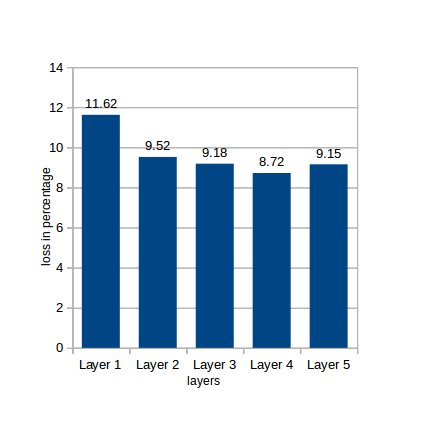
\includegraphics[scale=0.8]{figures/mlmkl_rand}
  \caption{Change in classifier performance on \textit{mnist-back-rand} dataset when adding layers iteratively.}
  \label{fig_mbr_layers}
\end{figure}

\begin{figure}
  \centering
  \captionsetup{justification=centering,margin=0.1cm}
  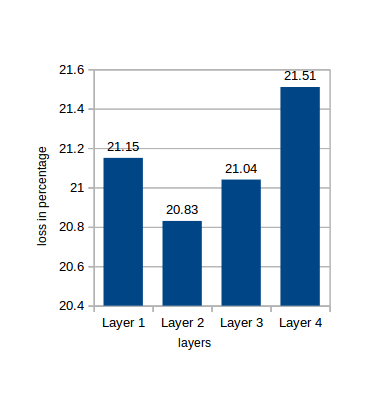
\includegraphics[scale=0.8]{figures/mlmkl_image}
  \caption{Change in classifier performance on \textit{mnist-back-image} dataset when adding layers iteratively.}
  \label{fig_mbi_layers}
\end{figure}

Figure \ref{tsne_rand_mlmkl} shows the tSNE embedding of the features learned by ML-MKL algorithm. The visualization indicates that classes are well separated.

\begin{sidewaysfigure}
  \centering
  \captionsetup{justification=centering,margin=0.1cm}
  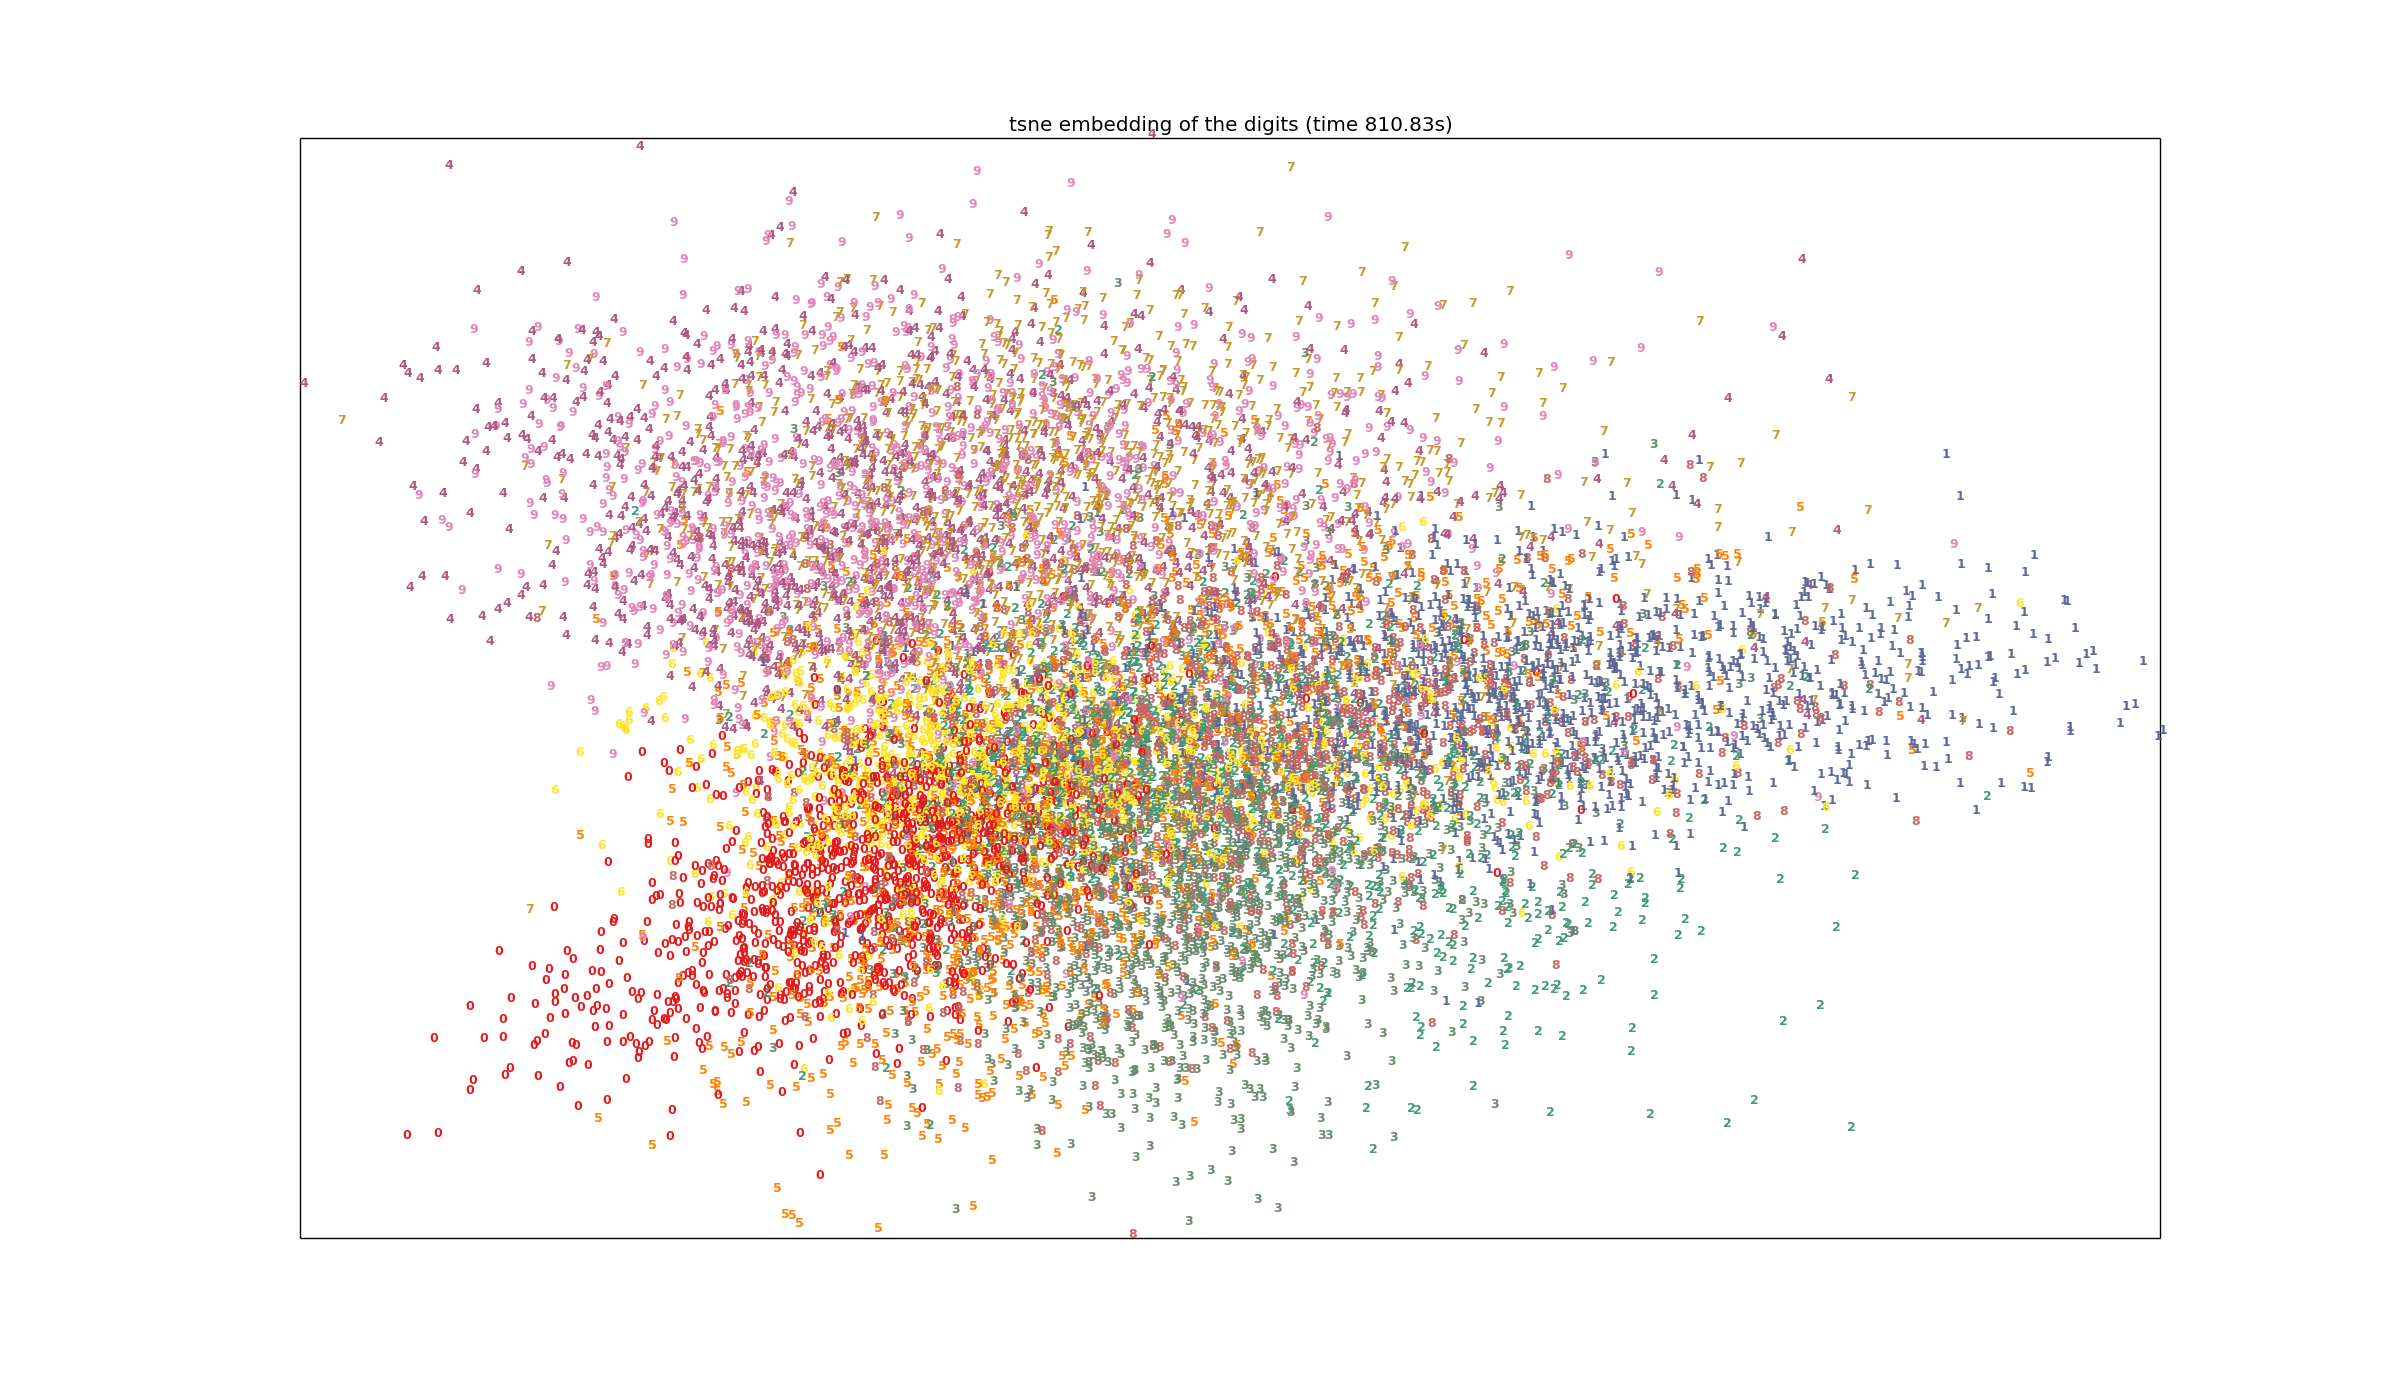
\includegraphics[scale=0.45]{figures/tsne_rand_mlmklbest}
  \caption{tSNE embedding of features obtained by ML-MKL algorithm for the \textit{mnist-back-rand} dataset.}
  \label{tsne_rand_mlmkl}
\end{sidewaysfigure}

Tables \ref{back_rand_kw} and \ref{back_image_kw} shows the kernel weights of each kernel in the mixture at every layer for \textit{mnist-back-rand} and \textit{mnist-back-image} datasets respectively. In both cases $k_1$ is an acr-cosine kernel, and the remaining are Gaussian kernels for \textit{mnist-back-rand} dataset and polynomial kernel for textit{mnist-back-image} dataset. The results in the table indicates that,  the contribution of individual kernels was highly varying in each layer (no single kernel had complete dominance over all layers in the feature learning process). 


\renewcommand{\arraystretch}{2.3}
\begin{table*}
\centering
\begin{tabular}{|c|c|c|c|c|c|c|c|}
  \hline
  \multirow{2}{*}{\textbf{Layers}} & \multicolumn{7}{ |c| }{\textbf{Kernel Weights}} \\
  \cline{2-8}
  & $k_1$ & $k_2$ & $k_3$ & $k_4$ & $k_5$ & $k_6$ & $k_7$ \\
  \hline  
  \textit{Layer 1} & 0.2007 & 0.1331 & 0.1331 & 0.1332 & 0.1332 & 0.1333 & 0.1333\\
  \hline
  \textit{Layer 2} & 0.2711 & 0.1160 & 0.1181 & 0.1203 & 0.1225 & 0.1248 & 0.1271\\
  \hline
  \textit{Layer 3} & 0.1764 & 0.0999 & 0.1125 & 0.1266 & 0.1426 & 0.1607 & 0.1811\\
  \hline
  \textit{Layer 4} & 0.0598 & 0.0524 & 0.0747 & 0.1071 & 0.1547 & 0.2245 & 0.3269\\
  \hline
  \textit{Layer 5} & 0.0514 & 0.0493 & 0.0726 & 0.1069 & 0.1569 & 0.2295 & 0.3334\\
  \hline    
\end{tabular}
\caption{Kernel weights in each layer for the \textit{mnist-back-rand} dataset}
\label{back_rand_kw}
\end{table*}
\renewcommand{\arraystretch}{1}

\renewcommand{\arraystretch}{2.3}
\begin{table}
\centering
\begin{tabular}{|c|c|c|c|c|c|}
  \hline
  \multirow{2}{*}{\textbf{Layers}} & \multicolumn{5}{ |c| }{\textbf{Kernel Weights}} \\
  \cline{2-6}
  & $k_1$ & $k_2$ & $k_3$ & $k_4$ & $k_5$\\
  \hline  
  \textit{Layer 1} & 0.2445 & 0.1887 & 0.1888 & 0.1889 & 0.1891\\
  \hline
  \textit{Layer 2} & 0.3421 & 0.1603 & 0.1630 & 0.1659 & 0.1688\\
  \hline
  \textit{Layer 3} & 0.2035 & 0.1615 & 0.1843 & 0.2104 & 0.2403\\
  \hline
  \textit{Layer 4} & 0.0843 & 0.1409 & 0.1877 & 0.2508 & 0.3362\\
  \hline
\end{tabular}
\caption{Kernel weights in each layer for the \textit{mnist-back-image} dataset}
\label{back_image_kw}
\end{table}
\renewcommand{\arraystretch}{1}

In order to evaluate the contribution of each kernel, exploratory analysis was carried out to monitor the performance of individual kernels in each layer. The individual kernels performance were compared with the combined kernel's performance. Tables \ref{back_rand_exp} and \ref{back_image_exp} summarizes the results of this exploratory analysis on \textit{mnist-back-rand} and \textit{mnist-back-image} datasets respectively (here $K_{conv}$ is the result of combined kernel). The results clearly indicates that the combination was not always improving the performance in all layers. However, the best result in both datasets were obtained by a combined kernel.

\renewcommand{\arraystretch}{2.1}
\begin{table*}
\centering
\begin{tabular}{|c|c|c|c|c|c|c|c|c|}
  \hline
  \multirow{2}{*}{\textbf{Layers}} & \multicolumn{8}{ |c| }{\textbf{Loss in Percentage}} \\
  \cline{2-9}
  & $k_1$ & $k_2$ & $k_3$ & $k_4$ & $k_5$ & $k_6$ & $k_7$ & $K_{conv}$\\
  \hline  
  \textit{Layer 1} & 11.46 & 9.92 & 10.06 & 10.04 & 10.1 & 9.87 & 10.06 & 11.62\\
  \hline
  \textit{Layer 2} & 10.36 & 9.87 & 9.90 & 9.89 & 9.92 & 9.82 & 9.81 & 9.52\\
  \hline
  \textit{Layer 3} & 9.46 & 11.07 & 10.33 & 9.85 & 9.70 & 9.56 & 9.01 & 9.18\\
  \hline
  \textit{Layer 4} & 9.26 & 9.06 & 8.95 & 8.96 & 8.93 & 8.72 & 9.00 & \textbf{8.72}\\
  \hline
  \textit{Layer 5} & 9.18 & 9.07 & 9.02 & 9.20 & 9.22 & 9.36 & 9.47 & 9.15\\
  \hline    
\end{tabular}
\caption{Individual kernels performance evaluation for \textit{mnist-back-rand} dataset}
\label{back_rand_exp}
\end{table*}
\renewcommand{\arraystretch}{1}

\renewcommand{\arraystretch}{2.1}
\begin{table}
\centering
\begin{tabular}{|c|c|c|c|c|c|c|}
  \hline
  \multirow{2}{*}{\textbf{Layers}} & \multicolumn{6}{ |c| }{\textbf{Loss in Percentage}} \\
  \cline{2-7}
  & $k_1$ & $k_2$ & $k_3$ & $k_4$ & $k_5$ & $K_{conv}$\\
  \hline  
  \textit{Layer 1} & 20.91 & 21.82 & 21.82 & 21.83 & 21.77 & 21.15\\
  \hline
  \textit{Layer 2} & 21.27 & 21.00 & 21.09 & 21.04 & 21.04 & \textbf{20.83}\\
  \hline
  \textit{Layer 3} & 20.95 & 21.18 & 21.02 & 20.99 & 21.05 & 21.03\\
  \hline
  \textit{Layer 4} & 21.06 & 21.36 & 21.42 & 21.64 & 21.66 & 21.51\\
  \hline
\end{tabular}
\caption{Individual kernels performance evaluation for \textit{mnist-back-image} dataset}
\label{back_image_exp}
\end{table}
\renewcommand{\arraystretch}{1}



\section{Conclusion}
\label{sec_conc}
In this chapter we explored the concept of multiple kernel learning in MKMs. A linear combination of multiple kernels formulated purely from unlabelled data is used in each layer of MKMs. The learning process of the proposed ML-MKL algorithm employs a greedy layerwise training for each layer. Empirical results indicates that using (unsupervised) MKL  in MKMs improves the classifier performance. In our experimental analysis the classification accuracy of ML-MKL models was better than learning machines with shallow architectures and was comparable with existing deep architectures.

Exploratory analysis performed on the features learned by the ML-MKL model reveals much more interesting facts about the model. The contribution of kernels in each layer is measured in terms of individual kernel performance and the weights assigned to that kernel. However this information is insufficient to determine the optimal structural complexity required for modelling a problem.
 % Confinement above
%\newpage
%\thispagestyle{empty}
%\mbox{}
\chapter{Kernel FDA with Multi-layer Kernels}
\label{chap_kfda}
In this chapter we study the discriminating power of multi-layer kernels with kernel Fisher Discriminant Analysis(KFDA\nomenclature{KFDA}{Kernel Fisher Discriminant Analysis}). The analysis in this section was done on binary classification problems. This chapter is organized as follows: section \ref{chap4_kfda} gives a brief introduction of kernel Fisher discriminant Analysis, section \ref{chap4_experiment} contains the results of empirical study on \textit{rectangles-image} and \textit{convex} datasets(both are binary classification problems studied extensively in deep learning literatures), and section \ref{chap4_conc} gives the conclusion.  

\section{Kernel Fisher Discriminant Analysis}
\label{chap4_kfda}
The working principle of discriminant analysis is to find a set of features that discriminates the classes very well(\cite{kfda} et al.). Fisher Discriminant Analysis(FDA) was originally proposed for learning a set of discriminating features in the input space. Kernel FDA is a non-linear generalization of FDA, in which the discriminating features are learned in feature space.

Let $X_1 = \{x_1^1, \ldots, x_{n_1}^1 \}$ and $X_2 = \{x_1^2, \ldots, x_{n_1}^2 \}$ be data samples from two classes (class 1 and class 2) and the union of two, denoted as $X = X_1 \cup X_2$ as the training set.  KFDA find the directions $f$ which maximizes the cost function

\begin{equation}
\mathcal{J}(f) = \frac{f^TS_B^{\phi}f}{f^TS_W^{\phi}f} 
\label{4_jw}
\end{equation}

where $f \in \mathcal{F}$ and $S_B^{\phi}$ and $S_W^{\phi}$ are the between and within class scatter matrices respectively
\[ S_B^{\phi} = (m_1^{\phi} - m_2^{\phi})(m_1^{\phi} - m_2^{\phi})^T \]
\[ S_W^{\phi} = \sum_{i=1,2}\sum_{x \in X_i} (\phi(x)-m_i^{\phi})(\phi(x)-m_i^{\phi})^T  \]
where $m_i^{\phi} = \frac{1}{n_i} \sum_{j=1}^{n_i} \phi(x_j^i)$. Intuitively maximizing $\mathcal{J}(f)$ is equivalent to finding a direction $w$ which maximizes the separation of the two classes while minimizing the within class variance(\cite{kfda} et al.). We need to transform the formulation in \ref{4_jw} in terms of kernel function $k(x, y) = \phi(x) \cdot \phi(y)$ in order to use kernels. According to RKHS\nomenclature{RKHS}{Reproducing Kernel Hilbert Space} theory, any solution to the Tikhnov regularization $f \in \mathcal{F}$ must lie in the span of the feature map($\phi(\cdot)$) corresponding to training examples. Thus it can be represented as
\begin{equation}
f = \sum_{i=1}^n \alpha_i \phi(x_i)
\label{4_wrkhs}
\end{equation}
combining \ref{4_wrkhs} and the definition of $m_i^{\phi}$ we have
\[ f^Tm_i^{\phi} = \frac{1}{n_i} \sum_{j=1}^n \sum_{k=1}^{n_i} \alpha_j k(x_j, x_k^i) = \alpha^T M_i \]
where $(M_i)_j = \frac{1}{n_i} \sum_{k=1}^{n_i}  k(x_j, x_k^i)$. Define $M = (M_1-M_2)(M_1-M_2)^T$. The we have
\begin{equation}
f^T S_B^{\phi} f = \alpha^T M \alpha
\label{4_wsbw}
\end{equation}
using similar transformations we have
\begin{equation}
f^T S_W^{\phi} f = \alpha^T N \alpha
\label{4_wsww}
\end{equation}
where $N = \sum_{i=1,2} K_i(I - \bm{1}_{n_i})K_i^T $, $K_i$ is an $n \times n_i$ matrix with entries $(K_i)_{nm} = k(x_n, x_m^i)$(this is the kernel matrix for class $i$), $I$ is the identity matrix and $\bm{1}_{n_i}$ is the matrix with with all entries $\frac{1}{n_i}$. The derivation of this compact forms $M$ and $N$ are shown in Appendix \ref{derivation2}.

Combining (\ref{4_wsbw}) and (\ref{4_wsww}) we will get an objective function in terms of $\alpha$.
\[ \mathcal{J}(\alpha) = \frac{\alpha^T M \alpha}{\alpha^T N \alpha}  \]
This problem can be solved by finding the leading eigen vectors of $N^{-1}M$. The projection of a new pattern $x$ onto $f$ is given by
\[ f \cdot \phi(x) = \sum_{i=1}^n \alpha_i k(x_i, x) \]
The estimation of $N \in \mathbb{R}^{n \times n}$ from a sample of size $n$ poses an ill-posed problem(since the sample size is not high enough to get an exact covariance structure in $\mathbb{R}^{n \times n}$). This problem is solved by replacing $N$ with $N_{\mu}$ as
\[ N_{\mu} = N + \mu I \]
where $\mu$ is a large positive constant and $I$ is the identity matrix. This has two possible benefits
\begin{itemize}
\item It makes the problem numerically more stable as for large $\mu$, $N_{\mu}$ will become positive definite.
\item It decreases the bias in sample based estimation of eigenvalues.
\end{itemize}


\section{Experiments}
\label{chap4_experiment}
Empirical study was conducted on two binary classification datasets namely \textit{rectangles-image} dataset and \textit{convex} dataset. A short description about \textit{rectangles-image} dataset is given in \autoref{chap_mkm}.
\subsection{Convex Dataset}
The \textit{convex} dataset consists of a single convex region in an image. The dataset was constructed by taking the intersection of a number of half-planes whose location and orientation were chosen uniformly at random. The classification task was to identify whether the shape enclosed in the image is convex or not. This dataset consists of 12000 training and 50000 testing samples of size 28$\times$28.

Figure \ref{shape} shows some sample images from \textit{rectangles-image} and \textit{convex} datasets. In the experiments, KFDA with multi-layer arc-cosine kernels were used for feature extraction and kNN classifier was used for the classification. Table \ref{kfda_results} shows the results of the empirical study.

\begin{figure*}
  \centering
  \captionsetup{justification=centering,margin=0.1cm}
  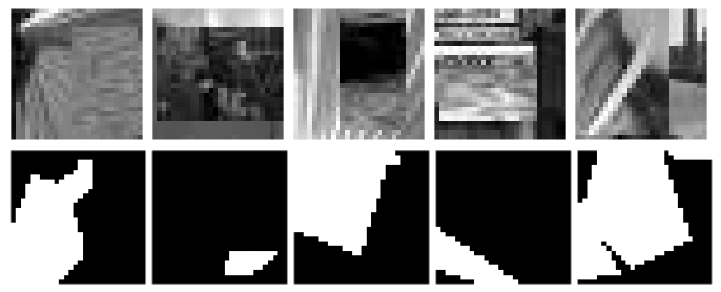
\includegraphics[scale=0.6]{figures/shapes}
  \caption{Sample images from \textit{rectangles-image}(first row) and \textit{convex}(second row) datasets.}
  \label{shape}
\end{figure*}

\renewcommand{\arraystretch}{2.3}
\begin{table*}
\centering
\begin{tabular}{|c|c|c|c|c|c|c|c|}
  \hline
  \multirow{2}{*}{\textbf{Dataset}} & \multicolumn{7}{ |c| }{\textbf{Loss in Percentage}} \\
  \cline{2-8}
  &$\textrm{SVM}_{\textrm{RBF}}$ & $\textrm{SVM}_{\textrm{Poly}}$ & NNet & DBN-3 & SAA-3 & DBN-1 & \textbf{KFDA}\\
  \hline  
  \textit{rect-image} & 24.04 & 24.05 & 33.20 & 23.69 & 24.05 & 22.50 & \textbf{21.96}\\
  \hline
  \textit{convex} & 19.13 & 19.82 & 32.25 & 19.92 & \textbf{18.41} & 18.63 & 19.02\\
  \hline
\end{tabular}
\caption{Experimental Results of KFDA with multi-layer kernels.}
\label{kfda_results}
\end{table*}
\renewcommand{\arraystretch}{1}

\renewcommand{\arraystretch}{2}
\begin{table}
\centering
\begin{tabular}{|c|c|}
  \hline
  \textbf{Kernel Parameters} &  \textbf{Loss in Percentage}\\
  \hline
  0 & 23.12\\
  \hline
  0,3 & 22.54\\
  \hline
  0,3,3 & 22.39\\
  \hline
  0,3,3,3 & 22.15\\
  \hline
  0,3,3,3,3 & 21.96\\
  \hline
  0,3,3,3,3,3 & 22.01\\
  \hline  
\end{tabular}
\caption{Change in classifier performance while increasing number of layers for \textit{rectangles-image} dataset}
\label{chap4_tab1}
\end{table}
\renewcommand{\arraystretch}{1}

\renewcommand{\arraystretch}{2}
\begin{table}
\centering
\begin{tabular}{|c|c|}
  \hline
  \textbf{Kernel Parameters} &  \textbf{Loss in Percentage}\\
  \hline
  1 & 21.94\\
  \hline
  1 $\times$ 3 & 21.68\\
  \hline
  1 $\times$ 6 & 21.46\\
  \hline
  1 $\times$ 9 & 19.78\\
  \hline
  1 $\times$ 12 & 19.52\\
  \hline
  1 $\times$ 15 & 19.38\\
  \hline
  1 $\times$ 18 & 19.30\\
  \hline
  1 $\times$ 21 & 19.02\\
  \hline      
\end{tabular}
\caption{Change in classifier performance while increasing number of layers for \textit{convex} dataset}
\label{chap4_tab2}
\end{table}
\renewcommand{\arraystretch}{1}

For \textit{rectangles-image} dataset, the best result was obtained for a five layer KFDA with kernel degree values in each layer was given by [0,3,3,3,3]. For \textit{convex} dataset the best result was obtained from a model having 20 layers with degree parameter equal to 1 in each layer. The variations in classifier performance as the number of layers were increased is shown in tables \ref{chap4_tab1} and \ref{chap4_tab2} for \textit{rectangles-image} and \textit{convex} datasets respectively. In table \ref{chap4_tab2}, 1 $\times$ $n$ indicates that an arc-cosine kernel of $n$ layers is used with kernel parameter is equal to `1' in each layer.


\section{Conclusion}
\label{chap4_conc}
In this chapter we experimented on KFDA with multi-layer arc-cosine kernels. The result obtained are very promising. On \textit{rectangles-image} dataset, the classifier performed even better than a DBN based model. On \textit{convex} dataset, its performance was better than all shallow models 
and was comparable with that of deep models. One of the striking observation from these results is that, better performance is obtained when using either a highly non-linear arc-cosine kernel(degree $>$ 1) or a multi-layer arc-cosine kernel with very large number of layers (above 10).
 % Confinement below

\chapter{Multi-layer Kernels in Structured Output Spaces}
\label{chap_struct}

This chapter focuses on evaluating multi-layer arc-cosine kernels on structured output prediction problems. The contents of this chapter are organized as follows; section \ref{chap5_intro} gives a brief description about the large margin formulation of pattern recognition problem on structured output spaces, section \ref{chap5_exp} talks about the result of empirical study on multi-class and multi-label classification problems and section \ref{chap5_conc} concludes the chapter.

\section{SVM in Structured Output Spaces}
\label{chap5_intro}
Typically machine learning algorithms are designed to produce flat real valued outputs; in the case of classification problems the output is a class label, for regression the output is a real number. For structured output learning algorithms, the output space has structured and interdependent variables, which is usually stored and processed as multi-dimensional arrays. For example, in the case of natural language parsing the output is a parse tree, in the case of image segmentation the output is the four 2D cordinates of bounding box surrounding the object. Two popular algorithms which works well in this domain are Conditional Random Fields(CRF\nomenclature{CRF}{Conditional Random Field}) proposed by \cite{crf} et al. and Structural SVMs proposed by \cite{joachims_struct} et al. In this project, we did our study on structural SVMs.

Structural SVMs are first introduced by \cite{joachims_struct} et al. in 2005, and  studied by \cite{joachims_cutting} et al. for simplifying the optimization problem while dealing with exponentially huge number of constraints. In particular, the number of constraints in the formulation of StructSVM is equal to the cardinality of the output space(which is exponential or even infinite). So decomposition methods like SMO\nomenclature{SMO}{Sequential Minimal Optimization} which process each constraints explicitly is not suitable for these kind of problems. \cite{joachims_cutting} et al. proved that the optimization problem can be solved efficiently using cutting plane algorithm proposed by \cite{cutting_plane}. They also proved that the number of iterations are independent of the number of training examples and provided an upper bound on the number of iterations.  

\subsection{StructSVM : Formulation}
Structured output prediction describes the problem of learning a function
\[ h: \mathcal{X} \longrightarrow \mathcal{Y} \]
where $\mathcal{X}$ is the input space and $\mathcal{Y}$ is the output space(structured). To learn $h$, we assume that a training sample of input-output pairs
\[ S = ((x_1, y_1), \ldots, (x_n, y_n)) \in (\mathcal{X} \times \mathcal{Y})^n \]
is available and drawn i.i.d from a joint distribution P($\mathcal{X},\mathcal{Y}$). Following empirical risk minimization principle, we will find an $h \in \mathcal{H}$ that minimizes the empirical risk
\[ R_s^{\bigtriangleup} = \frac{1}{n} \sum_{i=1}^n \bigtriangleup(y_i, h(x_i)) \]
Here $\bigtriangleup(y, \overline{y})$ denotes the \textbf{loss} associated with predicting $\overline{y}$ when $y$ is the correct output. The formulation assumes that the loss function is arbitrary and should satisfy the follwing requirments. 
\begin{equation*}
\bigtriangleup(y, \overline{y}) = 
\begin{cases}
 > 0 \textrm{ for } y \neq \overline{y} \\
 = 0 \textrm{ for } y = \overline{y}
 \end{cases}
\end{equation*}
StructSVM selects an $h \in \mathcal{H}$ that minimizes a regularized empirical risk on $S$. The general idea here is to learn a discriminant function $\mathnormal{f} : \mathcal{X} \times \mathcal{Y} \longrightarrow \mathbb{R}$ over input-output pairs from which one derives a prediction by maximizing $\mathnormal{f}$ over all $y \in \mathcal{Y}$ for a given input $x$.
\[ h_w(x) =  \underset{y \in \mathcal{Y}}{\arg\max} \mathnormal{f}_w(x,y) \]
We assume that $\mathnormal{f}_w(x,y)$ is linear in some combined feature space relating x and y, denoted as $\Psi(x,y)$.
\[ \mathnormal{f}_w(x,y) = (w \cdot \Psi(x,y)) \]
Here $w \in \mathbb{R}^N$ is the parameter vector. Intuitively we can think of $\mathnormal{f}_w(x,y)$ as a compatibility function that measures how well the output $y$ matches the given input $x$(\cite{joachims_cutting} et al.). This combined feature representation is required in the formulation, since we assumed that the sample $S$ is drawn from a joint distribution P($\mathcal{X},\mathcal{Y}$). Depending upon the structure of the output space, $\Psi(x,y)$ is defined separately for different problem instances.

\subsection{Margin Rescaling(MR) Formulation}
In order to take the loss into consideration, we modify the soft-margin formulation used in SVMs. The soft-margin formulation is given by
\[\underset{w, \xi \geq 0}{\min} \quad \frac{1}{2} \norm{w}^2 + \frac{C}{n} \sum_{i=1}^n \xi_i \]
\[ \textrm{s.t } \forall i \textrm{, } \forall \overline{y} \in \mathcal{Y}\setminus y_i \textrm{  :  } w^T[\Psi(x_i, y_i) - \Psi(x_i, \overline{y})] \geq 1 - \xi_i \textrm{, } \xi_i \geq 0 \]
Here $\xi_i$ is the slack variable and $C$ is the regularization parameter.
\[ \xi_i = \max\{ 0, \max_{y \in \mathcal{Y}\\y_i}(1 - w^T[\Psi(x_i, y_i) - \Psi(x_i, \overline{y})]) \} \]
As we have mentioned previously, this optimization problem is intractable for decomposition methods like SMO, since we have $\mathcal{O}(n|\mathcal{Y}|)$ constraints in the formulation. In Margin Rescaling\nomenclature{MR}{Margin Rescaling} formulation, the margin is adjusted according to the loss. In particular, we adjust the position of the hinge by keeping its slope fixed. The loss in MR formulation is computed as
\[ \bigtriangleup_{MR}(y, h_w(x)) =  \underset{\overline{y} \in \mathcal{Y}}{\max}\{ \bigtriangleup(y, \overline{y}) - (w^T[\Psi(x, y) - \Psi(x, \overline{y})]) \}  \textrm{ } \geq  \bigtriangleup(y, h_w(x))\]
and slack is obtained as $\xi = \max\{0, \bigtriangleup_{MR}(y, h_w(x))\}$. This leads to the following formulation
\[\underset{w, \xi \geq 0}{\min} \quad \frac{1}{2} \norm{w}^2 + \frac{C}{n} \sum_{i=1}^n \xi_i \]
\[ \textrm{s.t } \forall \overline{y_1} \in \mathcal{Y} \textrm{  :  } w^T[\Psi(x_1, y_1) - \Psi(x_1, \overline{y_1})] \geq \bigtriangleup(y_1, \overline{y_1}) - \xi_1 \]
\[ \vdots \]
\[ \textrm{s.t } \forall \overline{y_n} \in \mathcal{Y} \textrm{  :  } w^T[\Psi(x_n, y_n) - \Psi(x_n, \overline{y_n})] \geq \bigtriangleup(y_n, \overline{y_n}) - \xi_n \]
Intuitively, the constraints ensures that the score of the correct label $w^T\Psi(x_i, y_i)$ must be greater than all other scores $w^T\Psi(x_i, \overline{y_i}) \textrm{, } \forall \overline{y_i} \in \mathcal{Y} \setminus y_i$ by a required margin. In MR formulation, the margin is $\bigtriangleup(y_i, \overline{y_i})$.

\subsection{Slack Rescaling(SR) Formulation}
In Slack Rescaling\nomenclature{SR}{Slack Rescaling} formulation, the slack variables are rescaled according to the loss. In particular, the slope of the hinge loss function is adjusted while keeping its position fixed. In SR formulation the margin is 1. The loss in SR formulation is computed as
\[ \bigtriangleup_{SR}(y, h_w(x)) =  \underset{\overline{y} \in \mathcal{Y}}{\max}\{ \bigtriangleup(y, \overline{y})(1 - (w^T[\Psi(x, y) - \Psi(x, \overline{y})) \} \]
and slack is obtained as $\xi = \max\{0, \bigtriangleup_{SR}(y, h_w(x))\}$. This leads to the following formulation
\[\underset{w, \xi \geq 0}{\min} \quad \frac{1}{2} \norm{w}^2 + \frac{C}{n} \sum_{i=1}^n \xi_i \]
\[ \textrm{s.t } \forall \overline{y_1} \in \mathcal{Y} \textrm{  :  } w^T[\Psi(x_1, y_1) - \Psi(x_1, \overline{y_1})] \geq 1 - \frac{\xi_1}{\bigtriangleup(y_1, \overline{y_1})} \]
\[ \vdots \]
\[ \textrm{s.t } \forall \overline{y_n} \in \mathcal{Y} \textrm{  :  } w^T[\Psi(x_n, y_n) - \Psi(x_n, \overline{y_n})] \geq 1 - \frac{\xi_n}{\bigtriangleup(y_n, \overline{y_n})} \]
Both of the above formulation has n slack variables, hence it is called n-slack formulation. These formulations can be converted into 1-slack formulation by summing up all the slack variables(\cite{joachims_cutting} et al.). n-slack formumations have $\mathcal{O}(n|\mathcal{Y}|)$ constraints.

The solution space of this problem is a compact polyhedral convex set. The cutting plane algorithm finds the most violating constraint corresponding to each training example and add it to the working set. After each addition to the working set, we find a solution across all the constraints in working set. This effectively shrinks the size of the version space in a speedy manner. As the iteration continues, the number of constraint violations decreases and the algorithm converges. Every single cut in the convex set corresponds to a constraint violation. Instead of doing a step by step updation, the cutting plane algorithm cuts down a portion of the version space which results in faster convergence.
\section{Experiments} 
\label{chap5_exp}
Empirical study was conducted on multi-class and multi-label classification problems. For multi-class problems the loss function used was the absolute difference between labels, and for multi-label problems loss function was the hamming distance between labels expressed in binary form. Since the output space was finite, we used exhaustive search over $\mathcal{Y}$ in both cases, while finding the most violated constraints. Multi-label and multi-class classification problems are the simplest problem instances that can be studied using StructSVM, since their output space is finite.

The combined feature map $\Psi(x,y)$ was constructed as follows. Let $x \in \mathbb{R}^d$ and $k$ be the number of classes. Suppose $x$ is represented as $1:x_1, \ldots, d:x_d$. Then for multi-class problems $\Psi(x,y)$ was obtained by shifting the indices by $(y-1) \times d$ positions; i.e.,
\[ \Psi(x,y) = (y-1) \times d+1:x_1, \ldots, (y-1) \times d+d:x_d \]
For multi-label classification problems, we took the binary representation of $y$ and from that we extracted all bit positions that are ON. Then $\Psi(x,y)$ is computed by applying the same shifting to all the extracted indices.

Implementation was done using \cite{svm_struct} library, by modifying its API functions for multi-label and multi-class problems. Table \ref{chap5_tab1} lists the results of empirical study (value shown is the loss in percentage). The synthetic dataset was a multi-class problem instance available in \cite{svm_struct} library. Here the comparison was made between multi-layer (arc-cosine)kernel machines and commonly used single layer kernel machines.

\renewcommand{\arraystretch}{1.2}
\begin{table}
\centering
\begin{tabular}{|c|c|c|}
	\hline
	\textbf{Dataset} & \textbf{Arc-Cosine Kernel} & \textbf{Other Kernel(best)}\\
	\hline
	Scene Segentation & 30.35 & 30.60 \\
	(multilabel - 6 class) & & \\
	\hline
	Vehicle Dataset & 26.48 & 24.90 \\
	(multiclass - 4 class) & & \\
	\hline
	Iris Dataset & 1.67 & 3.33 \\
	(multiclass - 3 class) & & \\
	\hline
	Breast Cancer Wiscosin & 0.98 & 0.98 \\
	(binary) & & \\
	\hline
	Synthetic Data & 33.85 & 32.55 \\
	(multiclass - 7 class) & & \\
	\hline
\end{tabular}
\caption{Performance comparison of multi-layer arc-cosine kernel to other kernels in StructSVM framework.}
\label{chap5_tab1}
\end{table}
\renewcommand{\arraystretch}{1}

\section{Conclusion}
\label{chap5_conc}
In this chapter, we studied multi-layer kernels in structured output spaces. The experimental study was done on multi-label and multi-class problem instances. The results are competetive with single layer kernel machines. Multi-layer architectures are found to be effective in complex pattern recognition tasks. Hence the discriminating power of these multi-layer kernels must be tested in more complex structured output spaces on problems like natural language parsing, protein sequence alignment prediction etc.  
 %  Cylinder of varying cross section
\chapter{Conclusion and Future Works}
\label{chap_conc}
This thesis presents a study of deep multi-layer kernels on supervised and unsupervised learning algorithms. In the supervised learning settings, multi-layer kernels are studied on structured output prediction problems and discriminant analysis methods. In the unsupervised learning settings, multi-layer kernels are used for feature learning task. In particular, we used MKMs and MKL for building a feature learning framework with kernel machines whose architecture and training is equivalent to existing deep learning algorithms.

In the unsupervised feature learning model with MKMs we experimented with single kernel (arc-cosine kernel) and mixed kernels. In some cases, the mixed kernel version was found to be superior than their single kernel counterparts. Features learned by the MKMs were visualized with tSNE algorithm to understand the separability of different classes.

Instead of using single kernel in each layer, a convex combination of multiple kernels were tried out using an unsupervised MKL formulation. The training of this model was done in a greedy layer-by-layer fashion. Experimental results indicates that, this ML-MKL model is superior to single-kernel MKMs. Though we had conducted empirical study on object recognition datasets like \textit{cifar10} and text classification datasets like \textit{20-newsgroups}, the results were not very impressive. In the case of \textit{20-newsgroups} classification, multiple layers might be making the similarity information in the kernel matrix more noisy, since the performance was degrading after each layer is added.  The empirical studies on supervised learning settings also gave fruitful results. The KFDA algorithm with multi-layer kernels showed competitive performance with state of the art deep learning algorithms. Structured output learning algorithms also works well when multi-layer kernels were used.

\section{Future Works}
The empirical study conducted in this thesis is giving many insights, from which we can list out some potential future directions to explore.

The complexity of the model in terms of the number of layers and number of kernels in each layer are set by using  cross-validation techniques in our experiments. The optimal number of layers and optimal number of kernels in each layer characterizes the structure of ML-MKL. A thoretical study on the optimal structure of ML-MKL model is a future extension for this work.

The training of ML-MKL framework in the current implementation is performed in a greedy layer-by-layer fashion, by iteratively adding layers. This can be thought of as unsupervised pre-training done in typical deep learning algorithms. Then we can devise a supervised fine-tuning mechanism for this model, by taking class labels into account, which may change either the kernel parameters or weights.

The deep learning algorithms are found to be particularly effective for learning complex decision functions. Structured output prediction tasks like parse tree prediction, protein segment alignment prediction etc. need very complex decision functions. Thus, the deep multi-layer kernel machines can be studied in such domains.

The results from KFDA with multi-layer kernels is having some interesting aspects. The algorithm is performing well, either when using a highly non-linear arc-cosine kernel or when very large number of layers are used in the kernel function. The obscurity behind the need of such complex kernels for 
discriminant analysis can be explored further.
 %  Conclusion n future studies
%\input{Chapters/Chapter7} % 

%% ----------------------------------------------------------------
% Now begin the Appendices, including them as separate files


\appendix % Cue to tell LaTeX that the following 'chapters' are Appendices
\addtocontents{toc}{\vspace{2em}} % Add a gap in the Contents, for aesthetics

%\begin{appendices}
\chapter{Derivation of the objective function $J(\mu)$}
\label{derivation1}
The objective function to be minimized is given by
\[ \min_{k \in K_{conv}} \frac{1}{2}\sum_{i=1}^n \norm{x_i - \sum_{x_j \in B_i} k_{ij}x_j}^2 + \gamma* \sum_{i=1}^n \sum_{x_j \in B_i} k_{ij} \norm{x_i-x_j}^2 \]
Expanding the norm on the first part of the sum
\begin{equation}
\begin{split}
\min_{k \in K_{conv}} \frac{1}{2}\sum_{i=1}^n \bigg(\norm{x_i}^2 - 2*\sum_{x_j \in B_i} k_{ij} (x_i \cdot x_j)  + \\ k_i k_i^T \circ d_i d_i^T \circ X^TX \bigg) + \gamma* \sum_{i=1}^n \sum_{x_j \in B_i} k_{ij} \norm{x_i-x_j}^2
\end{split}
\label{new_obj}
\end{equation}
The notation `$\circ$' denotes elementwise multiplication of two vectors. Here the summation $\sum_{i=1}^n \norm{x_i}^2$ can be discarded, since it is independent of the optimization parameters. Substituting $X^TX = P$, 
\[\sum_{x_j \in B_i} k_{ij} (x_i \cdot x_j) = k_i \circ d_i \circ p_i\]
and 
\[ \sum_{x_j \in B_i} k_{ij} \norm{x_i-x_j}^2 = k_i \circ d_i \circ v_i \]
in \ref{new_obj} we will get the simplified objective function
\begin{equation}
\begin{split}
\min_{k \in K_{conv}} \sum_{i=1}^n \bigg( k_i k_i^T \circ d_i d_i^T \circ P + \\ 2\big(\gamma*k_i \circ v_i \circ d_i - k_i \circ p_i \circ d_i\big) \bigg)
\end{split}
\label{simplified}
\end{equation}
Here $p_i$ and $v_i$ are columns of $P$ and $M$ corresponding to $x_i$ respectively. Substituting $k_i = \sum_{t=1}^m \mu_tk_{t,i}$ in \ref{simplified} we will get
\[ \min_{\mu \in \Delta} \mu^T \Bigg( \sum_{t=1}^m \sum_{i=1}^n k_{t,i}k_{t,i}^T \circ d_i d_i^T \circ P \Bigg)^T \mu + z^T \mu \]
which is the objective function $J(\mu)$. Here $[z]_t = \sum_{i=1}^n (2 \gamma v_i \circ d_i - 2 p_i \circ d_i)^T \mathit{k}_{t,i} $ and $\mathit{k}_{t,i} = \Big[ k^t(x_i, x_1), \ldots, k^t(x_i, x_n) \Big]^T $ is the $i^{th}$ column of the $t^{th}$ kernel matrix.

\chapter{Derivation of cost function $\mathcal{J}(\alpha)$ in KFDA}
\label{derivation2}
The cost function is given as
\begin{equation}
\mathcal{J}(f) = \frac{f^TS_B^{\phi}f}{f^TS_W^{\phi}f} 
\label{b_jw}
\end{equation}
We have
\begin{equation}
f^Tm_i^{\phi} = \frac{1}{n_i} \sum_{j=1}^n \sum_{k=1}^{n_i} \alpha_j k(x_j, x_k^i) = \alpha^T M_i
\label{b_wmi}
\end{equation}
applying \ref{b_wmi} in the numerator of \ref{b_jw} we get
\begin{equation*}
\begin{aligned}
f^TS_B^{\phi}f &= f^T(m_1^{\phi} - m_2^{\phi})(m_1^{\phi} - m_2^{\phi})^Tf \\
&= (f^T m_1^{\phi}-f^Tm_2^{\phi}) \cdot (f^Tm_1^{\phi}-f^Tm_2^{\phi}) \\
&= (\alpha^T M_1 - \alpha^T M_2) \cdot (\alpha^T M_1 - \alpha^T M_2) \\
&= \alpha^T (M_1 - M_2)(M_1 - M_2)^T \alpha \\
&= \alpha^T M \alpha
\end{aligned}
\end{equation*}
where $M = (M_1-M_2)(M_1-M_2)^T$. Applying $f = \sum_{i=1}^n \alpha_i \phi(x_i)$ in the denominator of \ref{b_jw}
\begin{equation}
f^TS_W^{\phi}f = (\sum_{i=1}^n \alpha_i \phi(x_i))^T \sum_{j=1,2} \sum_{x \in X_j} (\phi(x)-m_j^{\phi})(\phi(x)-m_j^{\phi})^T (\sum_{i=1}^n \alpha_i \phi(x_i))
\label{b_wsw}
\end{equation}
To simplify the notations, define
\[ P_{ij} =  \sum_{x \in X_i} \phi(x_j) \cdot \phi(x) \]
Then 
\begin{equation}
\sum_{i=1}^n \sum_{j=1,2} \sum_{x \in X_j} \alpha_i(\phi(x_i) \cdot \phi(x)) = \alpha^TP_1 + \alpha^T P_2
\label{b_alphap}
\end{equation}
Applying \ref{b_alphap} in \ref{b_wsw} we get
\begin{equation*}
\begin{aligned}
f^TS_W^{\phi}f &= (\alpha^T P_1 - \alpha^T M_1) \cdot (\alpha^T P_1 - \alpha^T M_1) + (\alpha^T P_2 - \alpha^T M_2) \cdot (\alpha^T P_2 - \alpha^T M_2) \\
&= \alpha^T(P_1-M_1)(P_1-M_1)^T \alpha + \alpha^T(P_2-M_2)(P_2-M_2)^T \alpha \\
&= \alpha^T K_1(I - \bm{1}_{n_1})K_1^T \alpha + \alpha^T K_2(I - \bm{1}_{n_2})K_2^T \alpha \\
&= \alpha^T \Big(\sum_{i=1,2} K_i(I - \bm{1}_{n_i})K_i^T \Big) \alpha \\
&= \alpha^T N \alpha
\end{aligned}
\end{equation*}
where $K_j = \sum_{i=1}^n \sum_{x \in X_j} k(x_i, x)$, $I$ is the identity matrix, $\bm{1}_{n_j}$ is the matrix with with all entries $\frac{1}{n_j}$ and $N = \sum_{i=1,2} K_i(I - \bm{1}_{n_i})K_i^T$. Thus the cost function becomes
\[\mathcal{J}(f) = \frac{f^TS_B^{\phi}f}{f^TS_W^{\phi}f} = \frac{\alpha^T M \alpha}{\alpha^T N \alpha} \]
%\end{appendices}
	% Appendix Title

%\input{Appendices/AppendixB} % Appendix Title

%\input{Appendices/AppendixC} % Appendix Title

\addtocontents{toc}{\vspace{2em}}  % Add a gap in the Contents, for aesthetics
\backmatter

%% ----------------------------------------------------------------
%\label{Bibliography}
%\%lhead{\emph{Bibliography}}  % Change the left side page header 	to "Bibliography"
%\bibliographystyle{plain}  % Use the "unsrtnat" BibTeX style for formatting the Bibliography
%\bibliography{bibo}  % The references (bibliography) information are stored in the file named "Bibliography.bib"
\begin{thebibliography}{9}
\bibitem[Cho]{saul} Y. Cho, L.K. Saul, Kernel Methods  for Deep Learning.
\newblock \emph{Advances in Neural Information Processing Systems(NIPS)} Volume 22, 342 -- 350, 2009.

\bibitem[Bengio, 2007]{bengioAI} Yoshua Bengio and Yann LeCun, Scaling learning algorithms towards AI.  in Bottou, L. and Chapelle, O. and DeCoste, D. and Weston, J. (Eds) \newblock \emph{Large-Scale Kernel Machines}, MIT Press,  2007.

\bibitem[Bengio, 2013]{bengioRL} Yoshua Bengio, Aaron Courville and Pascal Vincent, Representation Learning: A Review and New Perspectives. \newblock \emph{IEEE Transactions on Pattern Analysis and Machine Intelligence(TPAMI)} Volume 35, 1798--1828, August 2013.

\bibitem[Bengio, 2009]{bengioLDA} Yoshua Bengio, Learning Deep Architectures for AI. \newblock \emph{Foundations and Trends in Machine Learning} Volume 2, 1 -- 127, January 2009.

\bibitem[Graham]{cifarBest}Benjamin Graham, Fractional Max-pooling. \newblock \emph{arxiv:cs/arXiv:1412.6071}, 2014.

\bibitem[Wan]{mnistBest} Li Wan, Matthew Zeiler, Sixin Zhang, Yann LeCun and  Rob Fergus, Regularization of Neural Networks using DropConnect. \newblock \emph{JMLR Proceedings} Volume 28, 1058 -- 1066, 2013.

\bibitem[Hinton 2012]{speechBest} Geoffrey Hinton, Li Deng, Dong Yu, George Dahl, Abdel-rahman Mohamed, Navdeep Jaitly, Andrew Senior, Vincent Vanhoucke, Patrick Nguyen, Tara Sainath and Brian Kingsbury, Deep Neural Networks for Acoustic Modeling in Speech Recognition. \newblock \emph{IEEE Signal Processing Magazine} Volume 29, 82 -- 97, 2012.

\bibitem[Alex]{imagenet} Alex Krizhevsky, Ilya Sutskever and Geoffrey E. Hinton, ImageNet Classification with Deep Convolutional Neural Networks. \newblock \emph{Neural Information Processing Systems(NIPS)}, 1106 -- 1114, 2012.

\bibitem[Collobert]{nlpBest} R. Collobert and J. Weston. A unified architecture for natural language processing: Deep neural networks with multitask learning. \newblock \emph{International Conference on Machine Learning(ICML)}, 2008.

\bibitem[Hinton, 2006]{hintonDBN} Geoffrey E. Hinton, Simon Osindero, and Yee Whye Teh, A fast learning algorithm for deep belief nets. \newblock \emph{Neural Computation}, 2006.

\bibitem[LeCun]{lecunnCNN} Yann LeCun, L\'{e}on Bottou, Yoshua Bengio and Patrick Haffner, Gradient based learning applied to document recognition. \newblock \emph{Proceedings of the IEEE}, 2278–2324,
November 1998.

\bibitem[Raina]{gpu1} Rajat Raina, Anand Madhavan and Andrew Y. Ng, Large-scale Deep Unsupervised Learning using Graphics Processors. \newblock \emph{International Conference on Machine Learning}, 2009.

\bibitem[Dean]{gpu2} Jeffrey Dean, Greg S. Corrado, Rajat Monga, Kai Chen, Matthieu Devin, Quoc V. Le, Mark Z. Mao, Marc’Aurelio Ranzato, Andrew Senior, Paul Tucker, Ke Yang and Andrew Y. Ng, Large Scale Distributed Deep Networks. \newblock \emph{Advances in Neural Information Processing Systems}, 1223 -- 1231, 2012.

\bibitem[Graphlab]{graphlab} Y. Low, J. Gonzalez, A. Kyrola, D. Bickson, C. Guestrin and J. Hellerstein, GraphLab: A New Framework For Parallel Machine Learning. \newblock \emph{26th Conference on Uncertainty in Artificial Intelligence (UAI)}, 2010.

\bibitem[Hugo]{dbn}Hugo Larochelle, Dumitru Erhan, Aaron Courville, James Bergstra, and Yoshua Bengio, Online companion for the paper An empirical evaluation of deep architectures on problems with many factors of variation. \newblock [Online]. Available: \url{http://www.iro.umontreal.ca/ ∼ lisa/twiki/bin/view.cgi/Public/DeepVsShallowComparisonICML2007} 2014.

\bibitem[Smola]{kpca} Bernhard Sch\"{o}lkopf, Alexander Smola and Klaus-Robert M\"{u}ller, Nonlinear Component Analysis As a Kernel Eigenvalue Problem. \newblock \emph{Journal of Neural Computation} Volume 10, 1299--1319, 1998.

\bibitem[Zhuang, 2011]{zhuang} J. Zhuang, Jialei Wang, Steven C.H Hoi, Xiangyang Lan, Unsupervised Multiple Kernel Learning. \newblock \emph{Journal of Machine Learning Research(JMLR)} Volume 20, 129--144, 2011.

\bibitem[Gert]{mkl} Gert R. G. Lanckriet, Nello Cristianini, Peter L. Bartlett, Laurent El Ghaoui, and Michael I. Jordan, Learning the kernel matrix with semidefinite programming. \newblock \emph{Journal of Machine Learning Research}, Volume 5, 27--72, 2004.

\bibitem[scikit-learn]{scikit} F. Pedregosa, G. Varoquaux, A. Gramfort, V. Michel, B. Thirion, O. Grisel, M.Blondel, P. Prettenhofer, R. Weiss, V. Dubourg, J. Vanderplas, A. Passos, D. Cournapeau, M. Brucher, M. Perrot, and E. Duchesnay, Scikit-learn: Machine Learning in Python. \newblock \emph{Journal of Machine Learning Research(JMLR)} Volume 12, 2825--2830, 2011.

\bibitem[MNIST]{mnist} Y. LeCun and C. Cortes, The MNIST database of handwritten digits. \newblock \url{http://yann.lecun.com/exdb/mnist/}.

\bibitem[Maaten]{tsne} L.J.P. van der Maaten and G.E. Hinton, Visualizing High-Dimensional Data Using t-SNE. \newblock \emph{Journal of Machine Learning Research(JMLR)}, volume 9, 2579--2605, 2008. 

\bibitem[Tsochantaridis]{joachims_struct} I. Tsochantaridis, T. Joachims, T. Hoffman and Y. Altun, Large Margin Methods for Structured and Interdependent Output SPaces. \newblock \emph{Journal of Machine Learning Research(JMLR) 6}, 1453--1484, 2005.

\bibitem[Joachims]{joachims_cutting} T. Joachims, T. Finely, C. John Nu, Cutting-Plane Training on Structural SVMs. \newblock \emph{Journal of Machine Learning 77(1)}, 27--59, 2009.

\bibitem[Kelley]{cutting_plane} J.E Kelley, The Cutting-plane Method for Solving Convex Programs. \newblock \emph{Journal of the Society for Industrial and Applied Mathematics(SIAM) 8}, 703--712, 1960.

\bibitem[Zhuang]{2l_mkl} Jinfeng Zhuang, Ivor W. Tsang and Steven C.H. Hoi, Two-layer Multiple Kernel Learning. \newblock \emph{International Conference on Artificial Intelligence and Statistics (AISTATS)}, pp 909--917, 2011. 

\bibitem[Ilyes]{deep_mkl} Ilyes Rebai, Yassine BenAyed and Walid Mahdi, Deep Multilayer Multiple Kernel Learning. \newblock \emph{Journal of Neural Computing and Applications}, pp 1--10, 2015.

\bibitem[Corinna]{corinna}Corinna Cortes, Mehryar Mohri, and Afshin Rostamizadeh, Two-stage learning kernel algorithms. \newblock \emph{International Conference on Machine Learning}, pp 239--246, 2010.

\bibitem[Sebastian]{kfda} Sebastian Mika, Gunnar R\"{a}tsch, Jason Weston, Bernhard Sch\"{o}lkopf, and Klaus-Robert M\"{u}ller, Fisher Discriminant Analysis With Kernels. \newblock \emph{Journel of Neural Networks for Signal Processing}, pp 41--48, 1999.

\bibitem[Lafferty]{crf} J. Lafferty, A. McCallum, and F. Pereira, Conditional random fields: Probabilistic models for segmenting and labeling sequence data. \newblock \emph{International Conference on Machine Learning}, 2001.

\bibitem[$\textrm{SVM}^{\textrm{struct}}$]{svm_struct} Thorsten Joachims, $\textrm{SVM}^{\textrm{struct}}$: Support Vector Machine for Complex Outputs. \newblock \url{http://www.cs.cornell.edu/People/tj/svm_light/svm_struct.html}
\end{thebibliography}


\clearpage
\addcontentsline{toc}{section}{\bf Source Code}
\section*{Source Code}
All the code-works done as part of this project is publicly hosted in github. The source code is available in the following repository\\
\url{https://github.com/akhilpm/Masters-Project/}
\vspace{4 em}
%\begin{center}
\addcontentsline{toc}{section}{\bf List of Papers based on thesis}
\section*{\bf List of papers based on thesis}
%\end{center}

\vspace{5 mm}
%1. Akhil P M, Asharaf S, Sumitra S, {\em Unsupervisd MKL in Multi-layer Kernel Machines}, Conference Name, Place, Status\\
1. Akhil P M, Asharaf S, Sumitra S, {\em Unsupervisd MKL in Multi-layer Kernel Machines}(paper under preparation).
\vspace{2 em}
\end{document}  % The End
%%	 ----------------------------------------------------------------
